\documentclass{article}

\usepackage{graphicx}
\usepackage{enumitem}

\begin{document}

% Nama Kelompok : Kelompok 1
% Kelas : D4 TI 1A
% 1. Dezha Aidil Martha ()
% 2. M.Tomy Maulidy ()
% 3. Habib Abdul Rasyid (1174002)
% 4. Nico Eklessia Sembiring (1174096)
% 5. Damara Benedikta Siolemba ()
% 6. Felix Setiawan Lase ()

\section{Pengertian Sensor Cahaya}

\begin{figure}[ht]
	\centerline{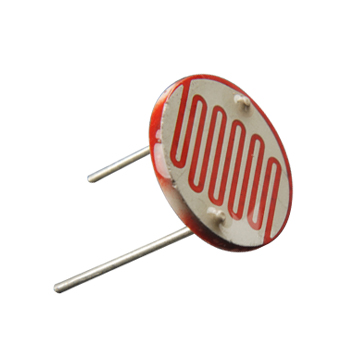
\includegraphics[width=0.4\textwidth]{figures/LDR.jpg}}
	\caption{LDR}
	\label{LDR}
\end{figure}

Sensor cahaya atau LDR merupakan sensor yang di pakai untuk mengubah besaran listrik menjadi besaran cahaya atau pengertian lain adalah  sensor yang membuat kita dapat melakukan pendeteksian cahaya, dan melakukan perubahan terhadap cahaya tersebut ,jadi sinyal listrik dan dipakai dalam sebuah rangkaian yang menggunakan cahaya sebagai alat pemicunya. Prinsip-prinsip kerja dari alat tersebut adalah untuk mengubah suatu energi dari foton menjadi elektron. Idealnya satu foton dapat membangkitkan satu elektron. Sensor cahaya sangat banyak penggunaannya, salah satu yang paling populer adalah kamera digital. Pada saat ini sudah ada alat yang digunakan untuk mengukur cahaya yang mempunyai 1 buah foton saja.

\section{Karakteristik Sensor Cahaya atau LDR}

Sensor Cahaya LDR (Light Dependent Resistor) merupakan suatu bentuk komponen yang mempunyai perubahan resistansi yang besarnya tergantung pada cahaya. Karakteristik LDR terdiri dari dua macam yaitu yang pertama Laju Recovery dan Respon Spektral.

Karakteristik sensor LDR adalah sebagai berikut :

\begin{itemize}
	\item LDR tipe arus harganya lebih besar dari 200K/detik.
	\item tidak mempunyai sensitivitas yang sama untuk setiap panjang gelombang cahaya yang jatuh padanya (yaitu warna).
	\item Dalam keadaan gelap resistansi LDR seki-tar 10MΩ dan dalam keadaan terang sebe-sar 1KΩ atau kurang.
\end{itemize}

\section{Cara Mengakses Sensor Cahaya}

\hspace{4mm} Bahan-bahan yang diperlukan untuk mengakses sensor Cahaya, yaitu :

\begin{itemize}
	\item Arduino Uno 
	\item Komputer + Software IDE Arduino
	\item Sensor LDR
	\item Kabel Jumper
	\item Lampu LED
	\item Kabel USB
	\item resistor
	\item breadboard
\end{itemize}

\break Proses pembuatan :

\begin{enumerate}
	
	\item  Pertama, pasang kabel biru ke bredboard -1 lalu di arduino ke slot power GND atas.
	\break
	\centerline{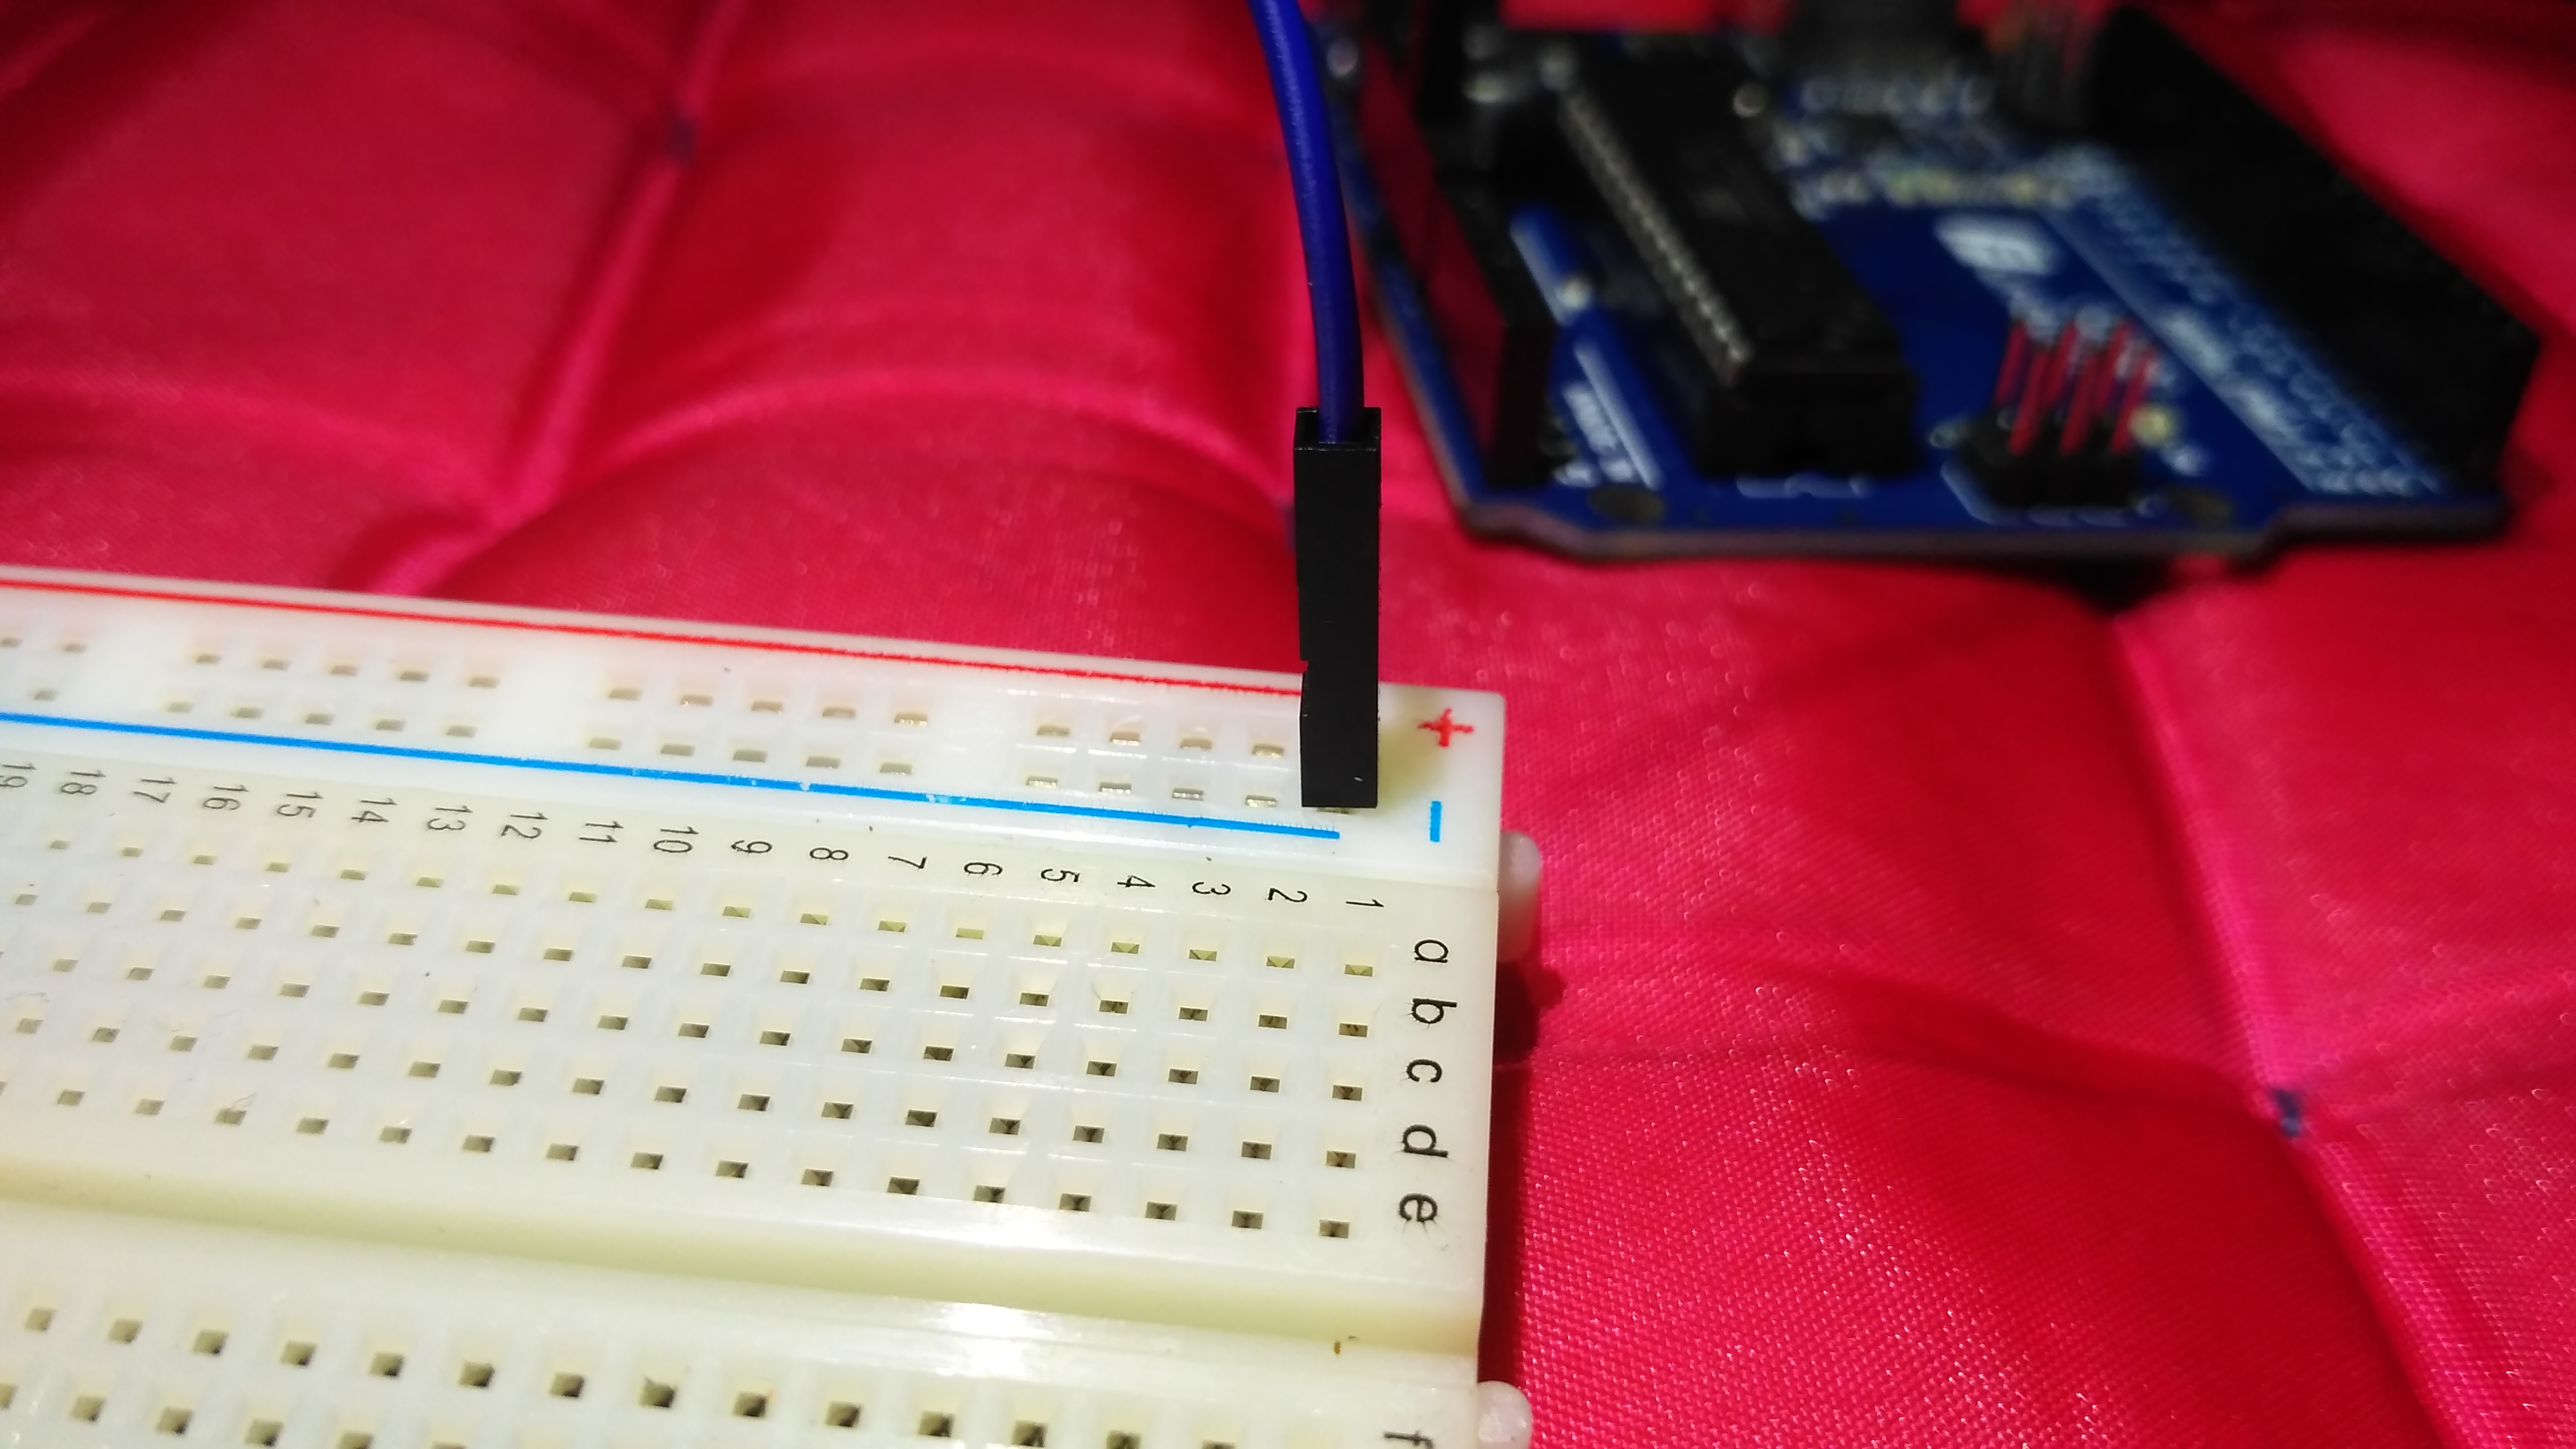
\includegraphics[width=0.9\textwidth]{figures/1.jpg}}
	\break
	\centerline{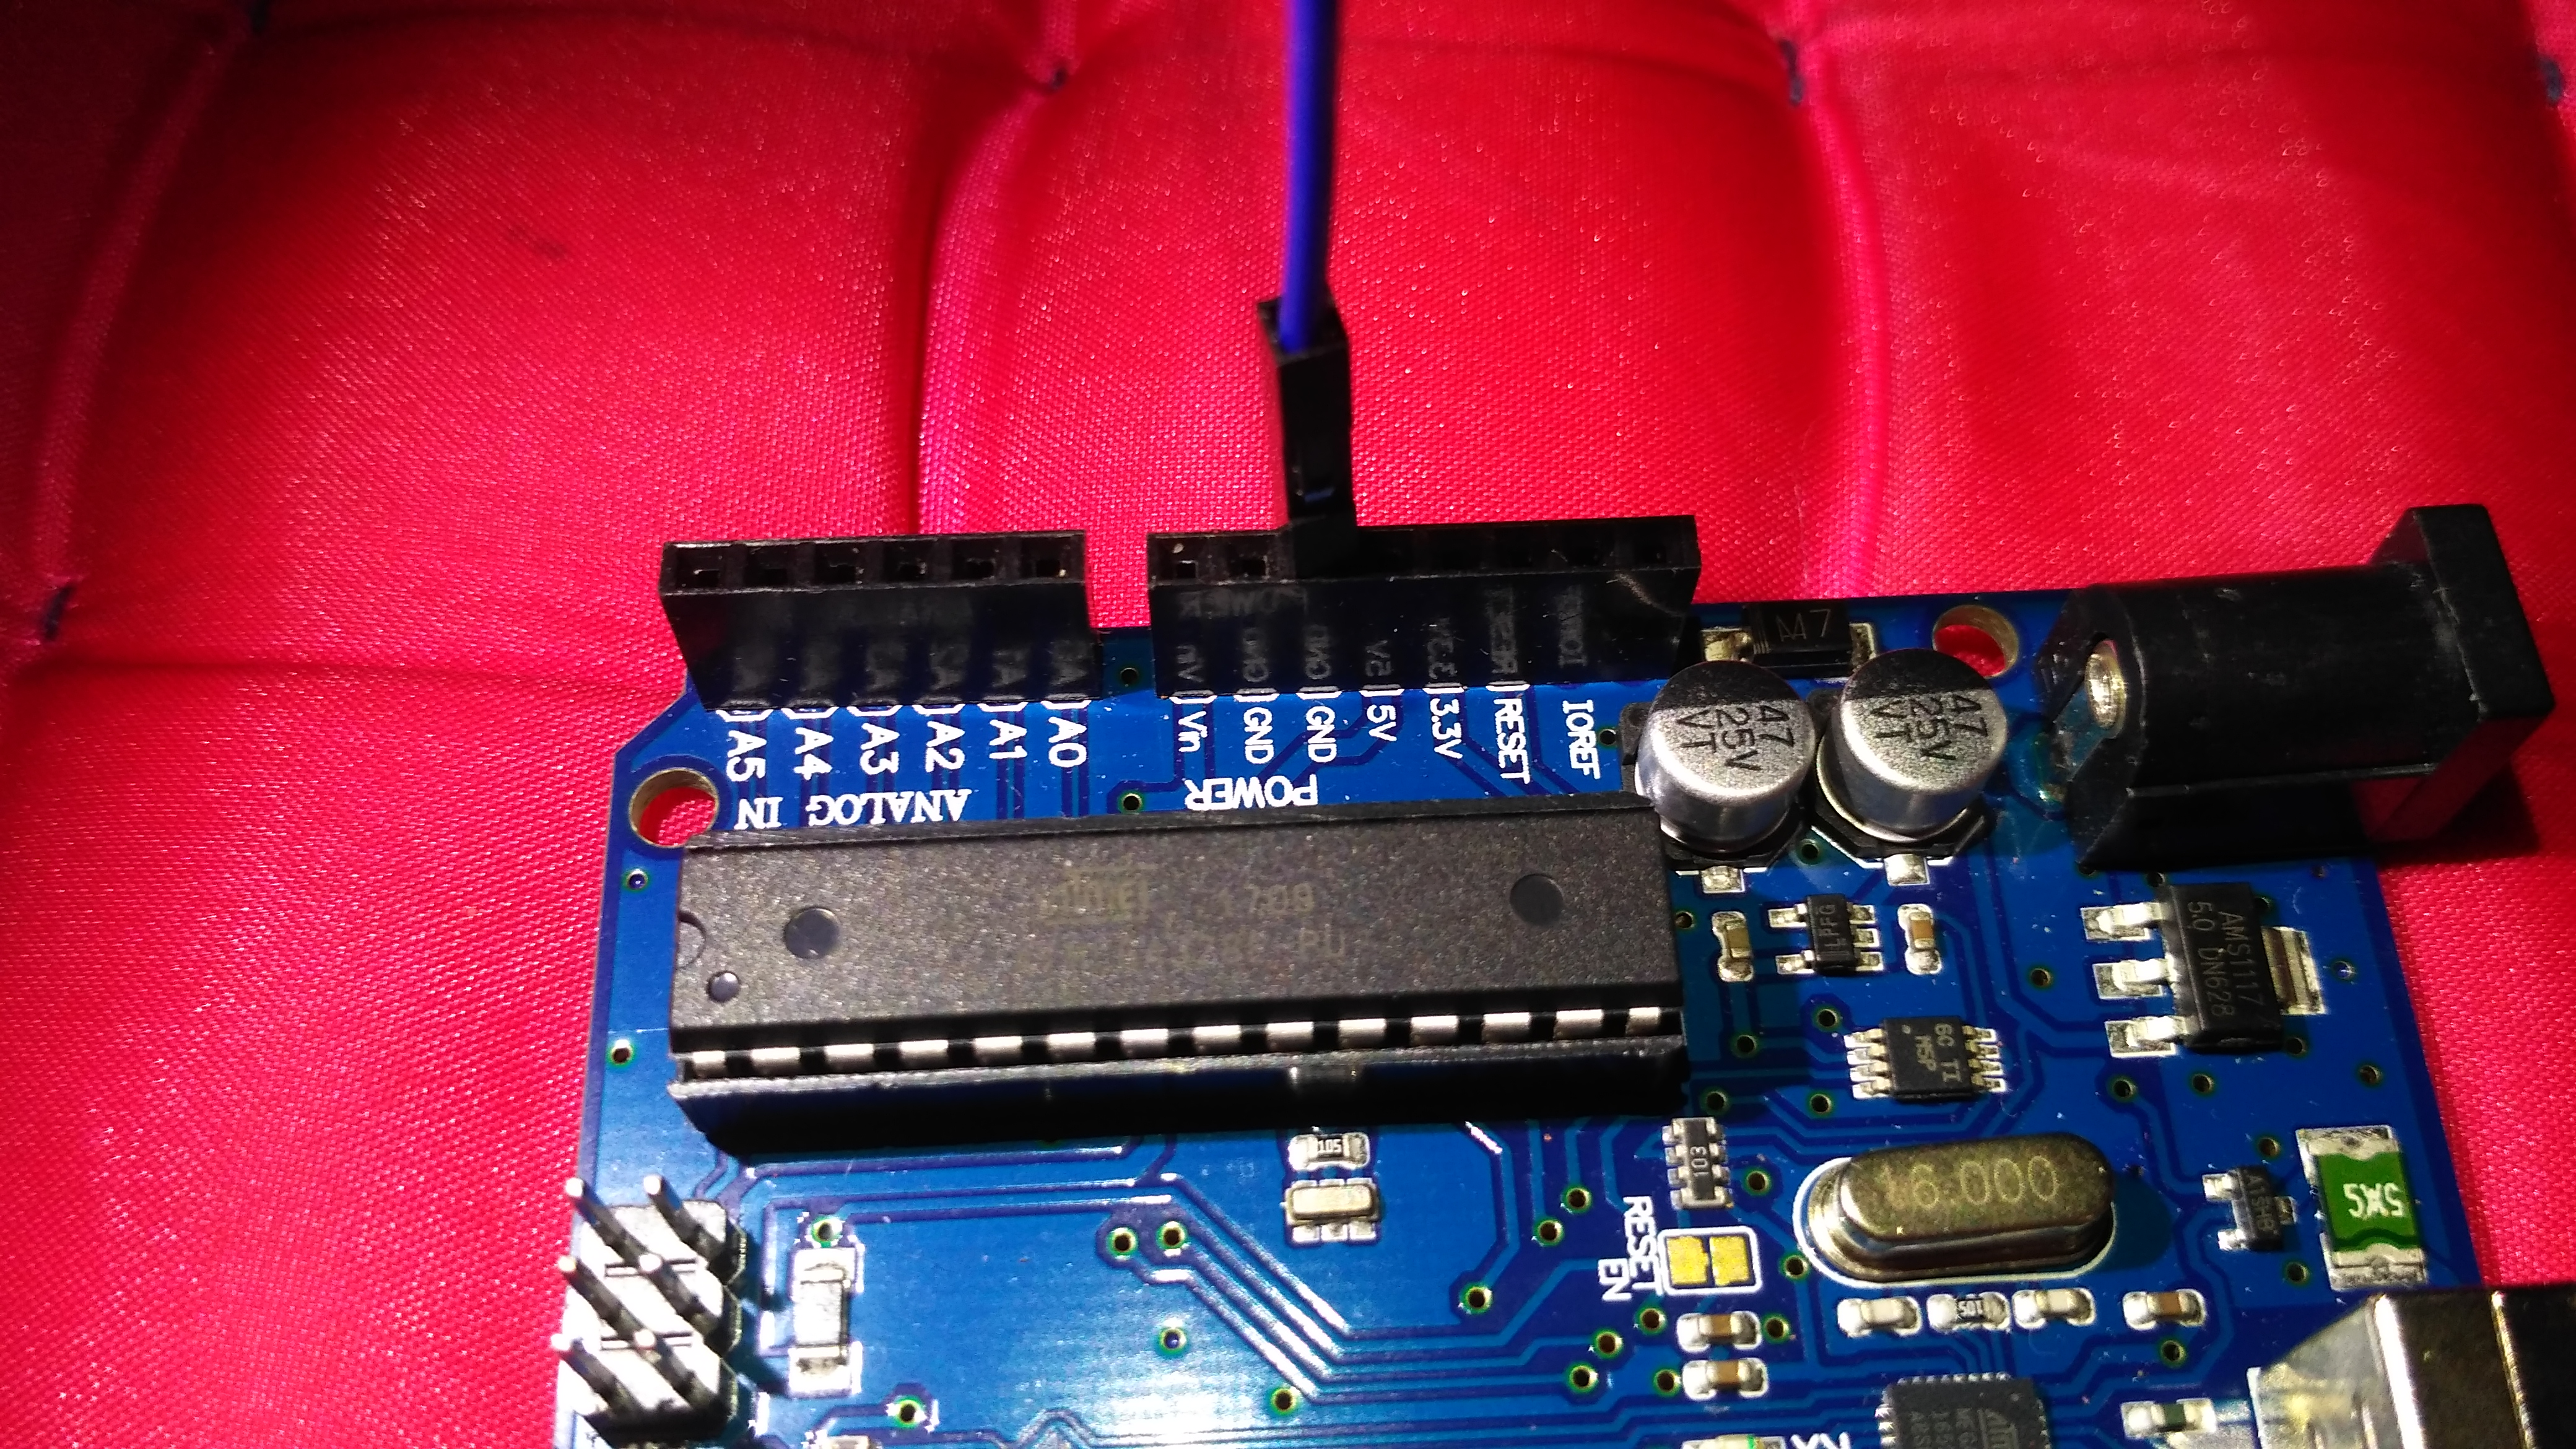
\includegraphics[width=0.9\textwidth]{figures/2.jpg}}
	\break
	\item Setelah semuanya terpasang, lalu kabel merah ke breadboard + 1 dan di aruduino ke slot Power 5V.
	\break
	\centerline{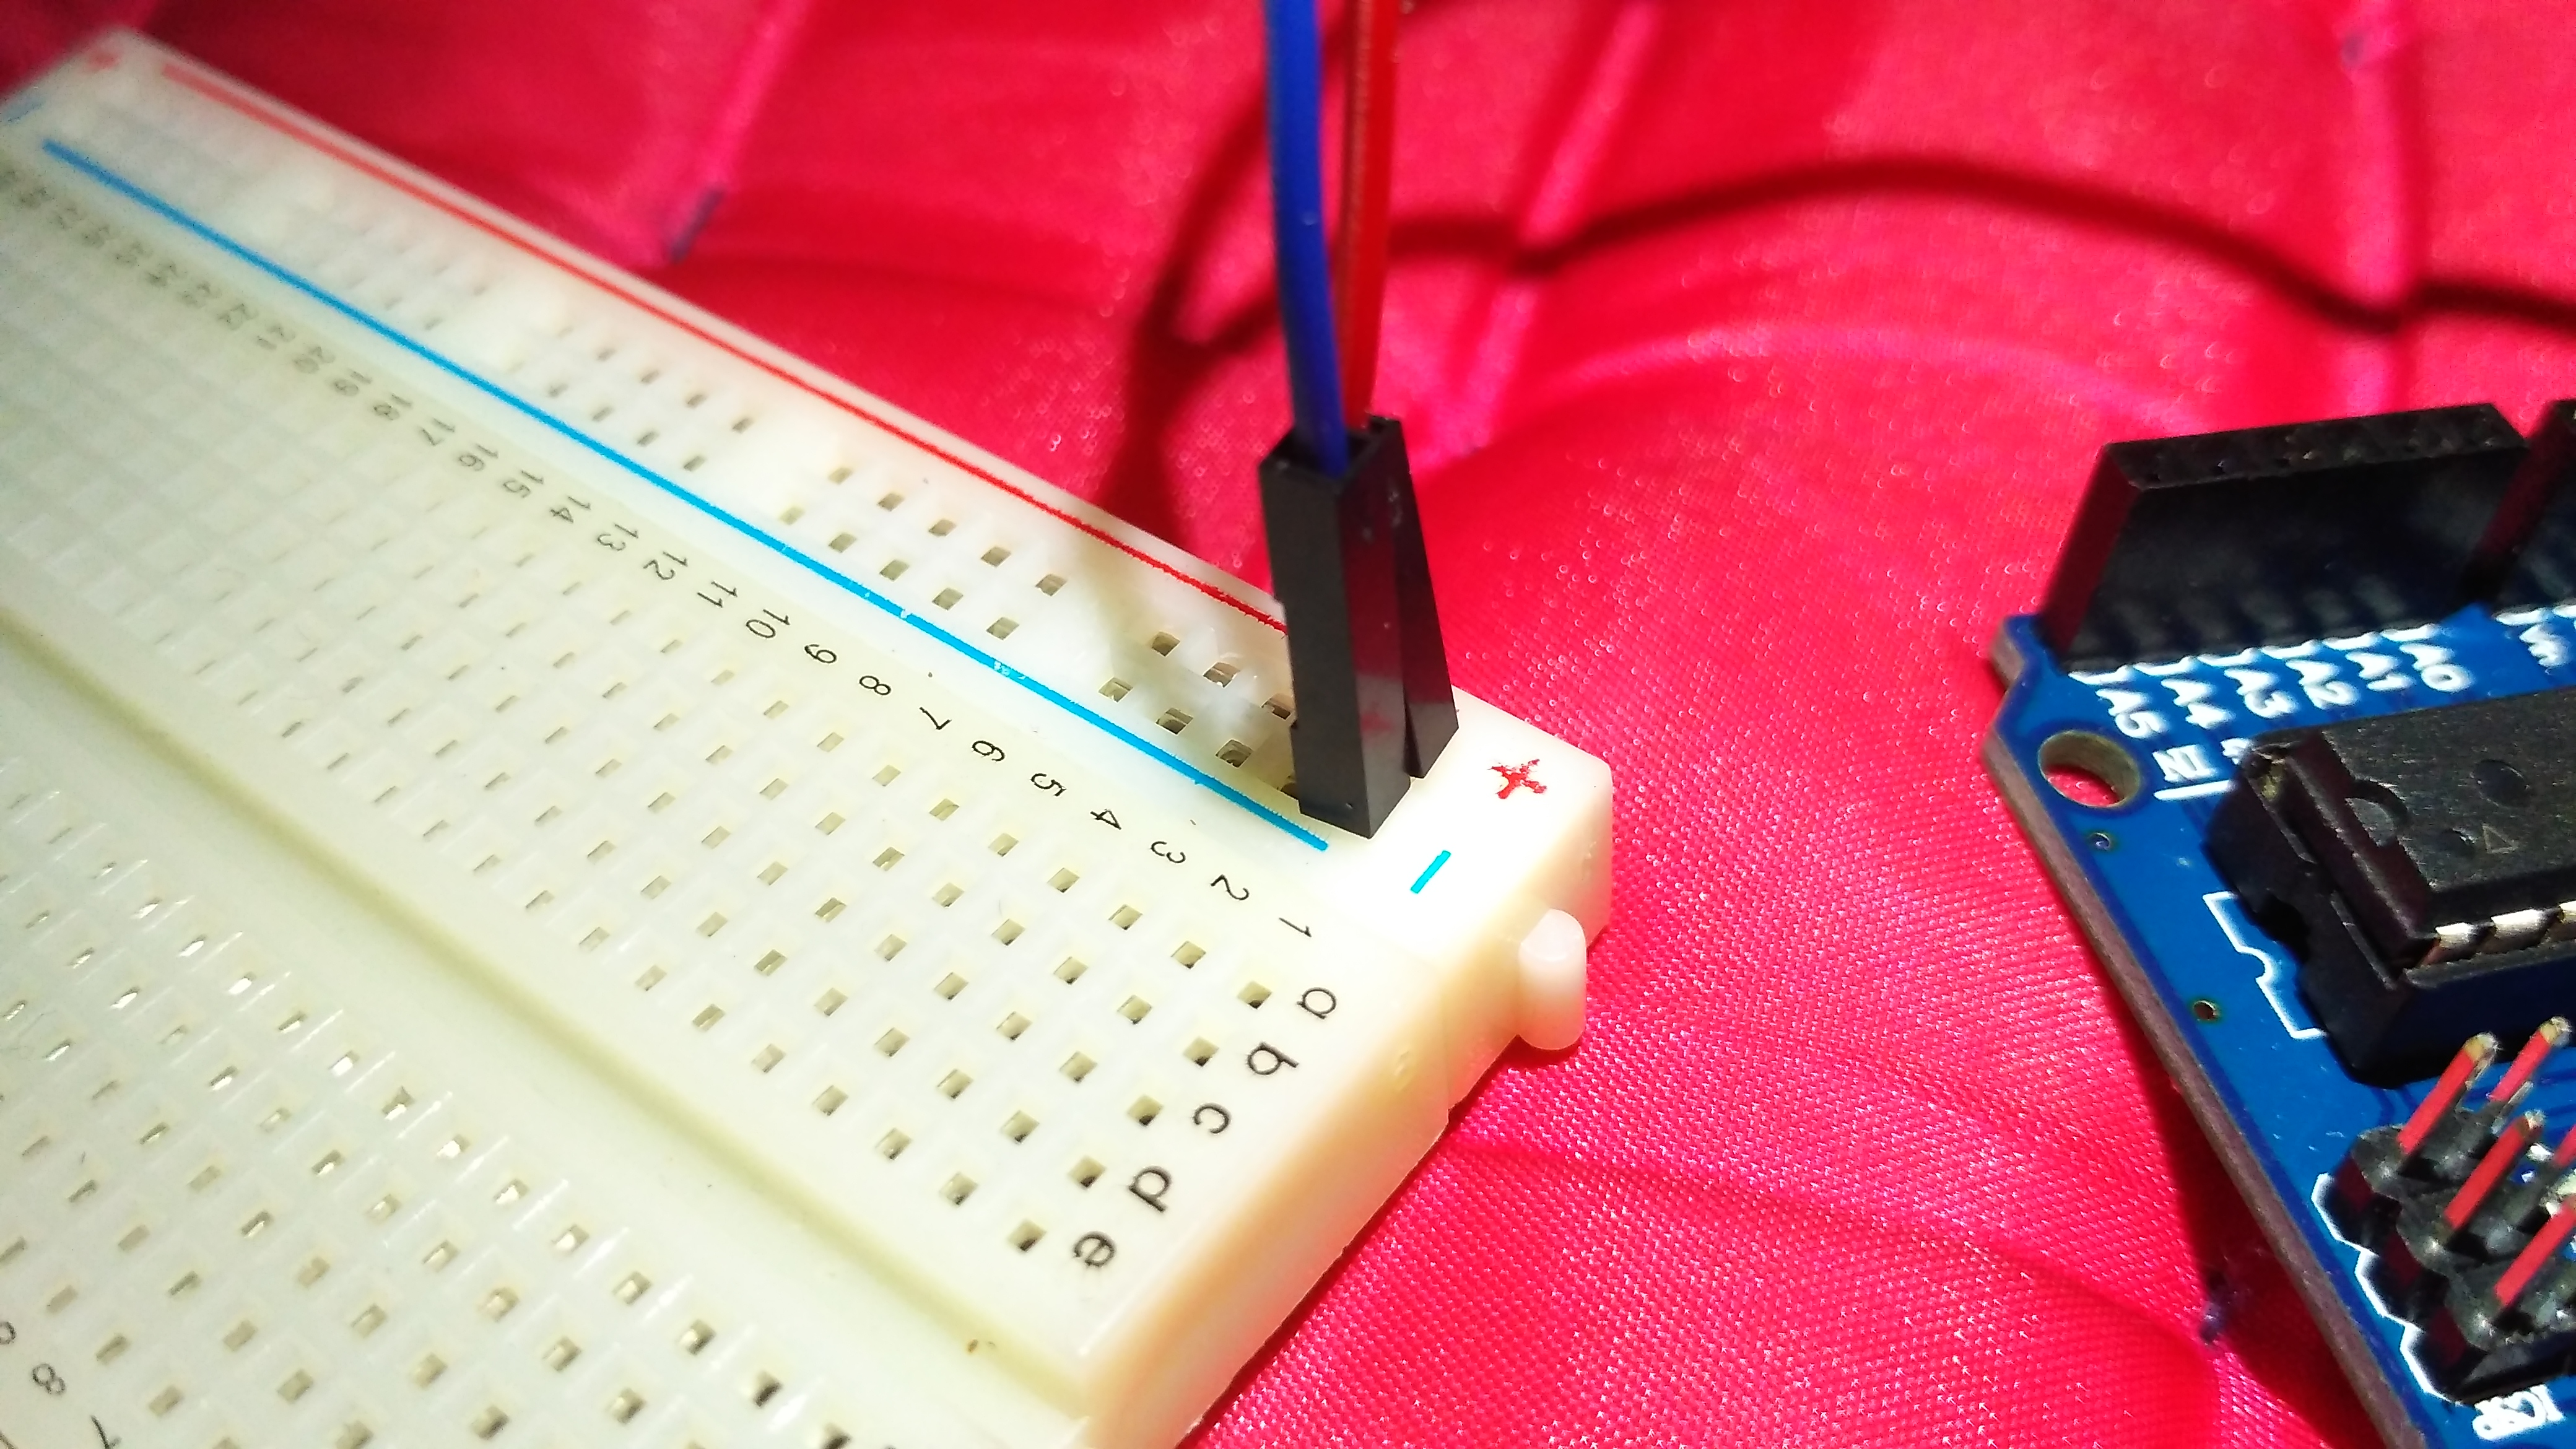
\includegraphics[width=0.9\textwidth]{figures/3.jpg}}
	\break
	\centerline{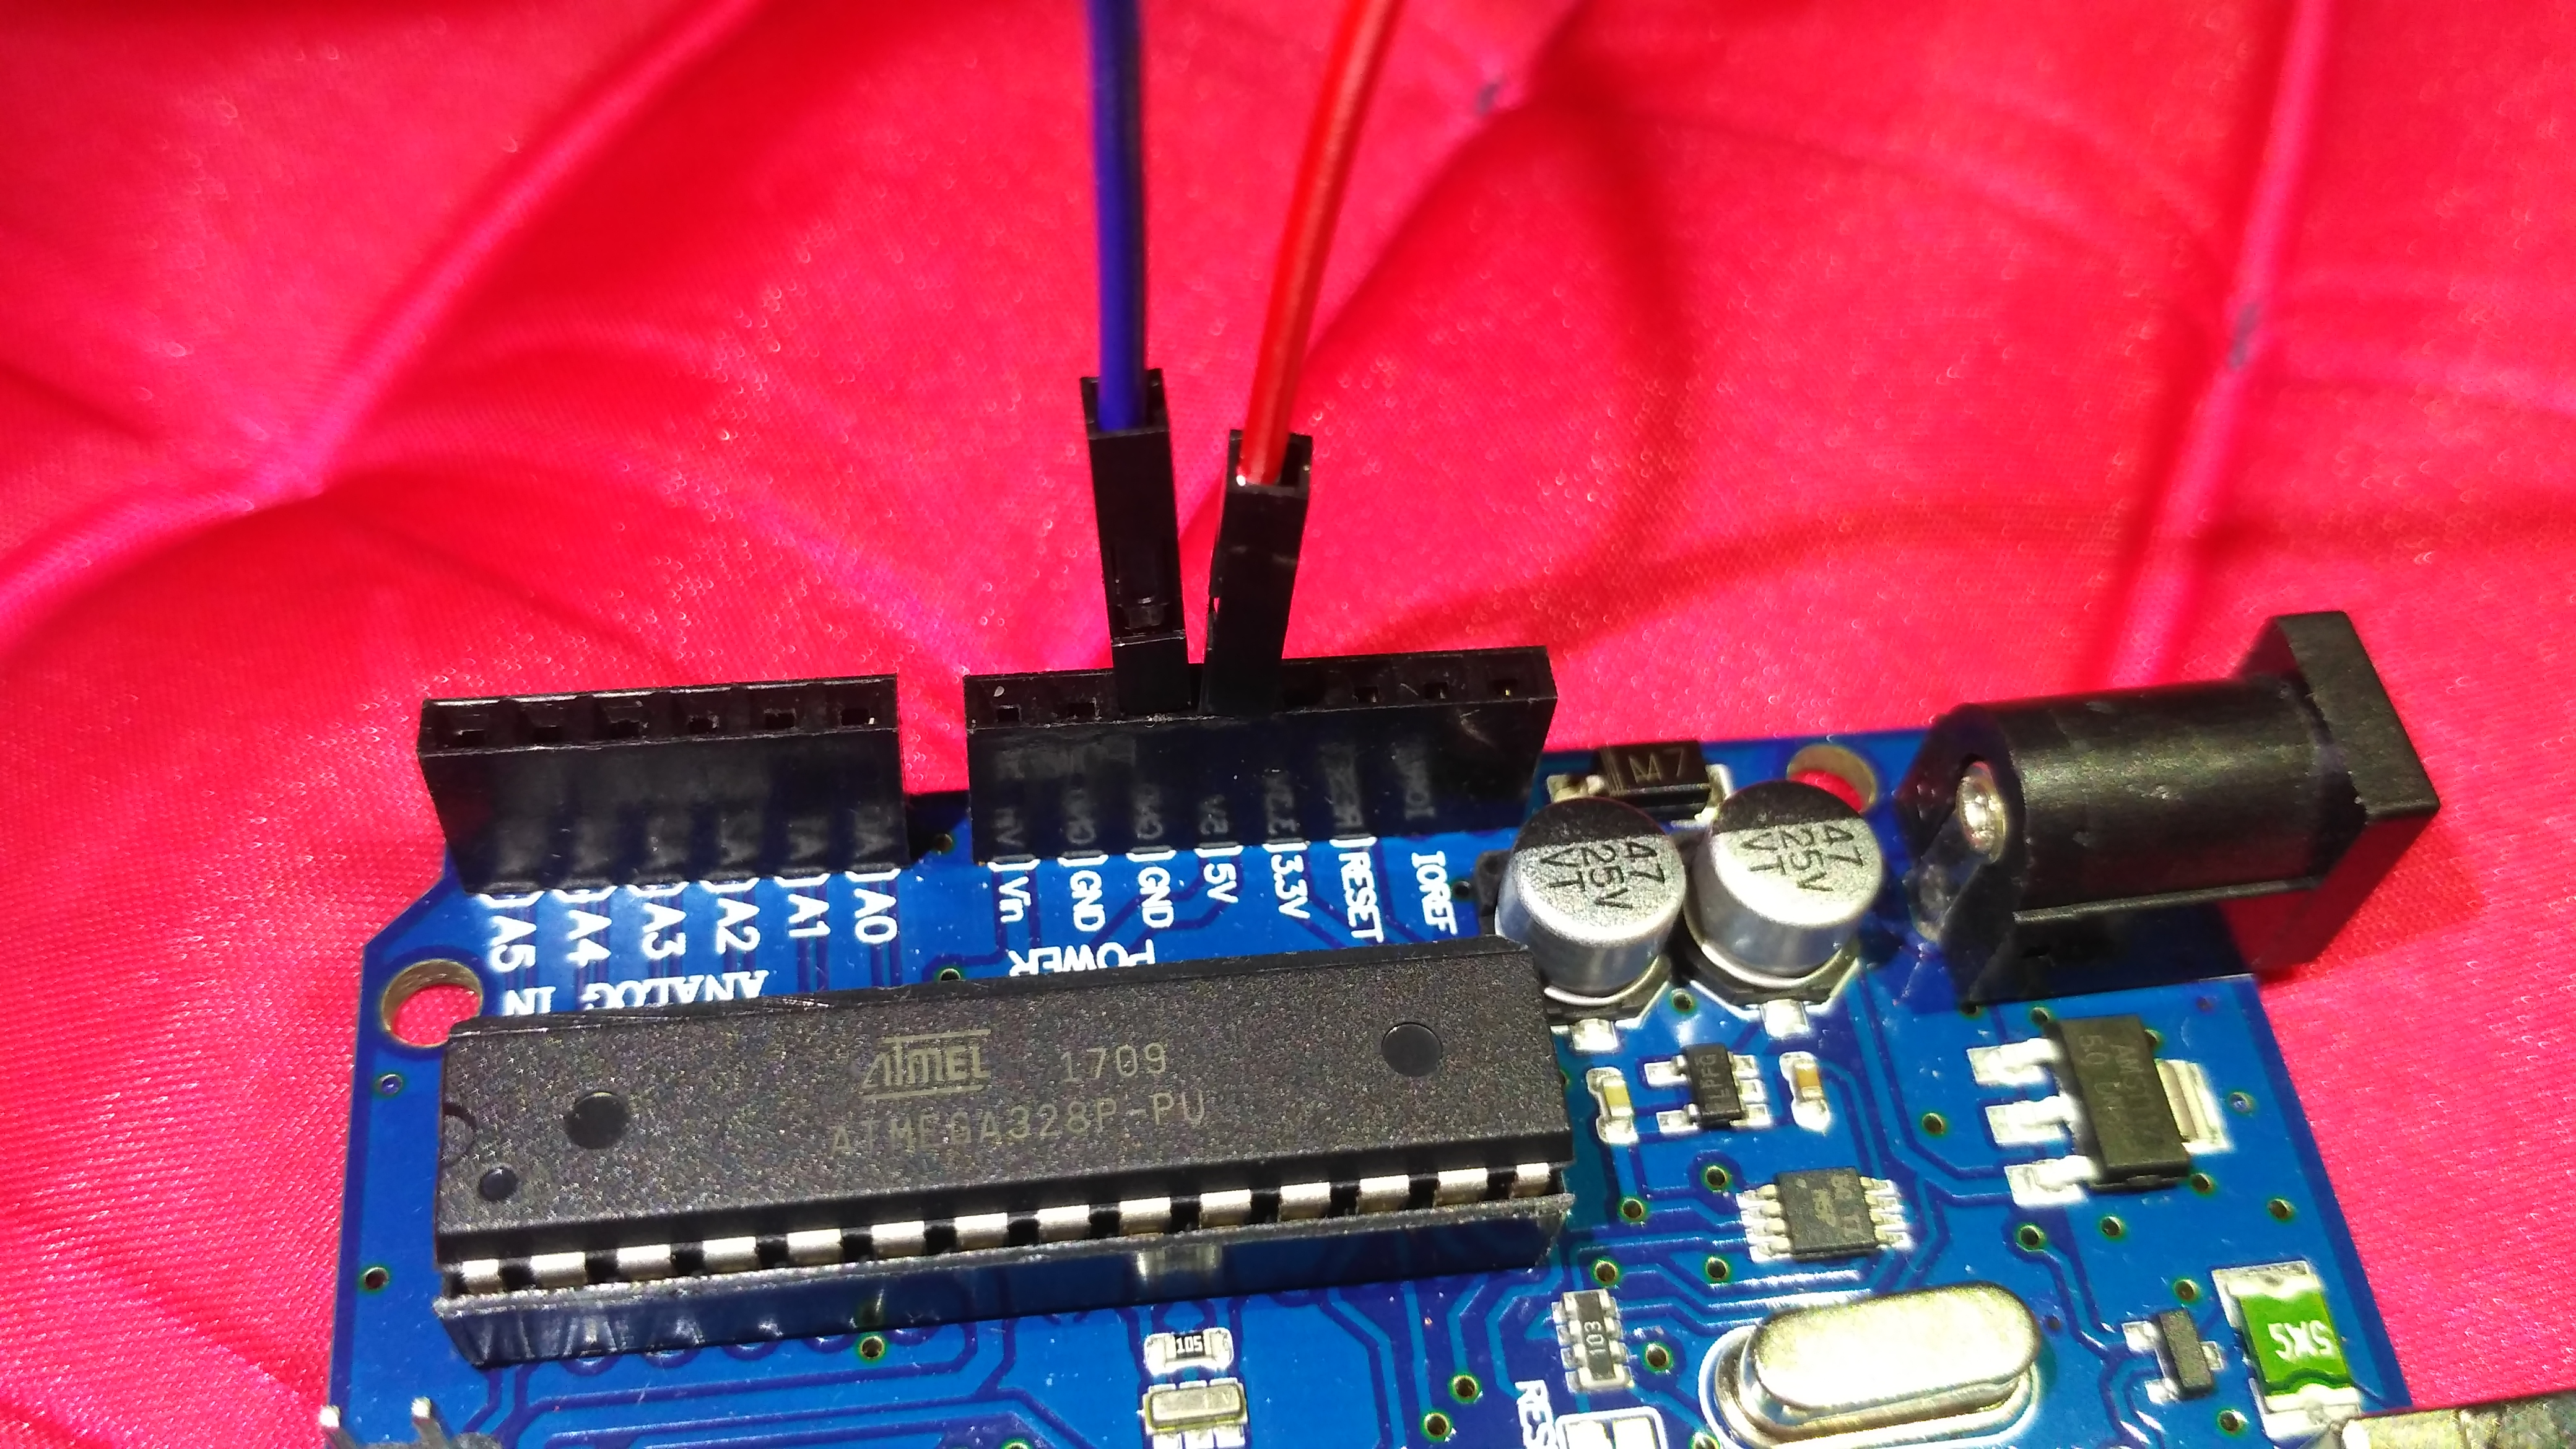
\includegraphics[width=0.9\textwidth]{figures/4.jpg}}
	\break
	\item pasangkan sensor LDR pada breadboard j12 dan j16.
	\break
	\centerline{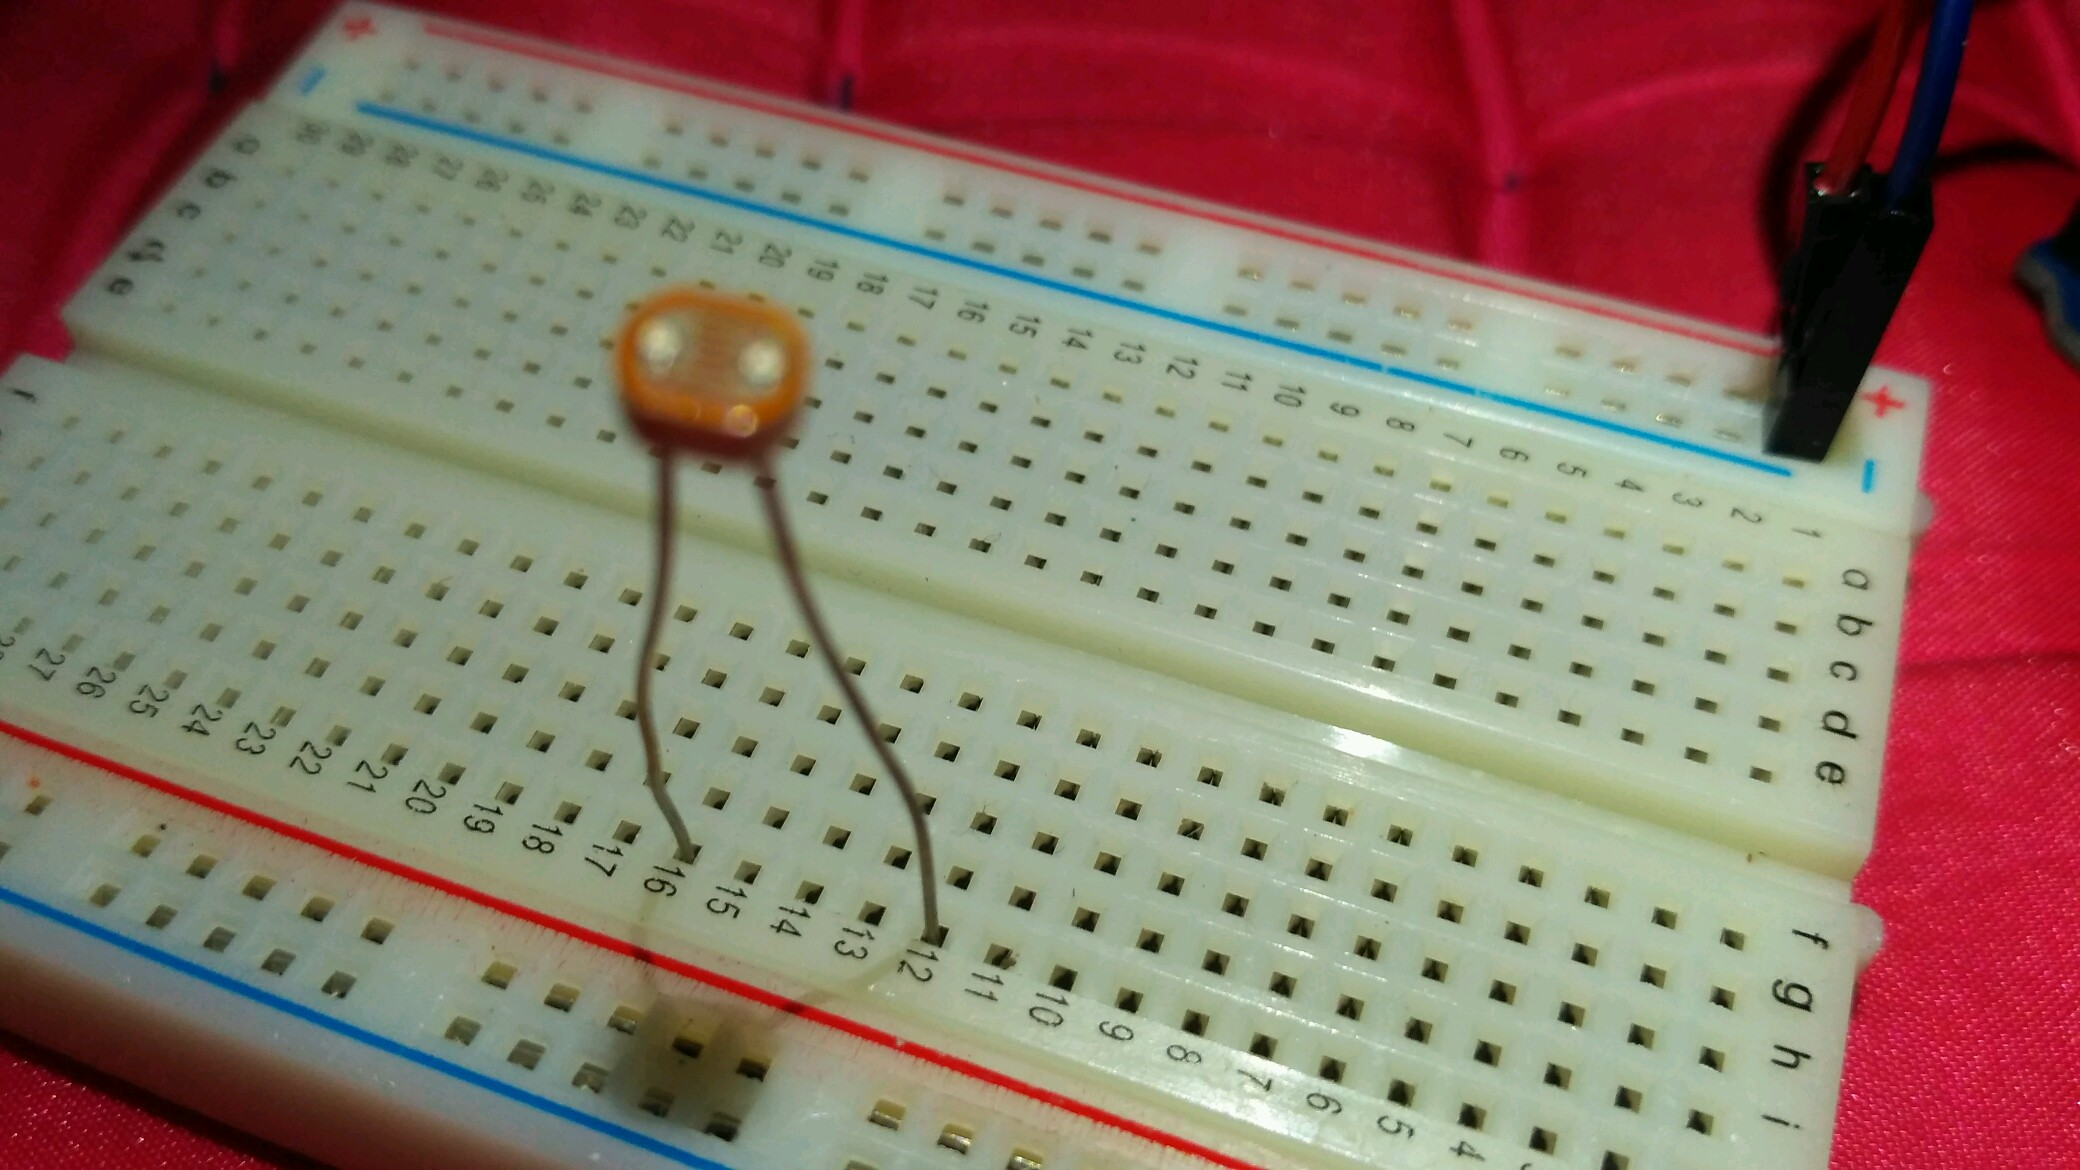
\includegraphics[width=0.9\textwidth]{figures/5.jpg}}
	\break
	\item Lalu pasang kabel orange 1 ke bredboard h12 ke bredboard +11.
	\break
	\centerline{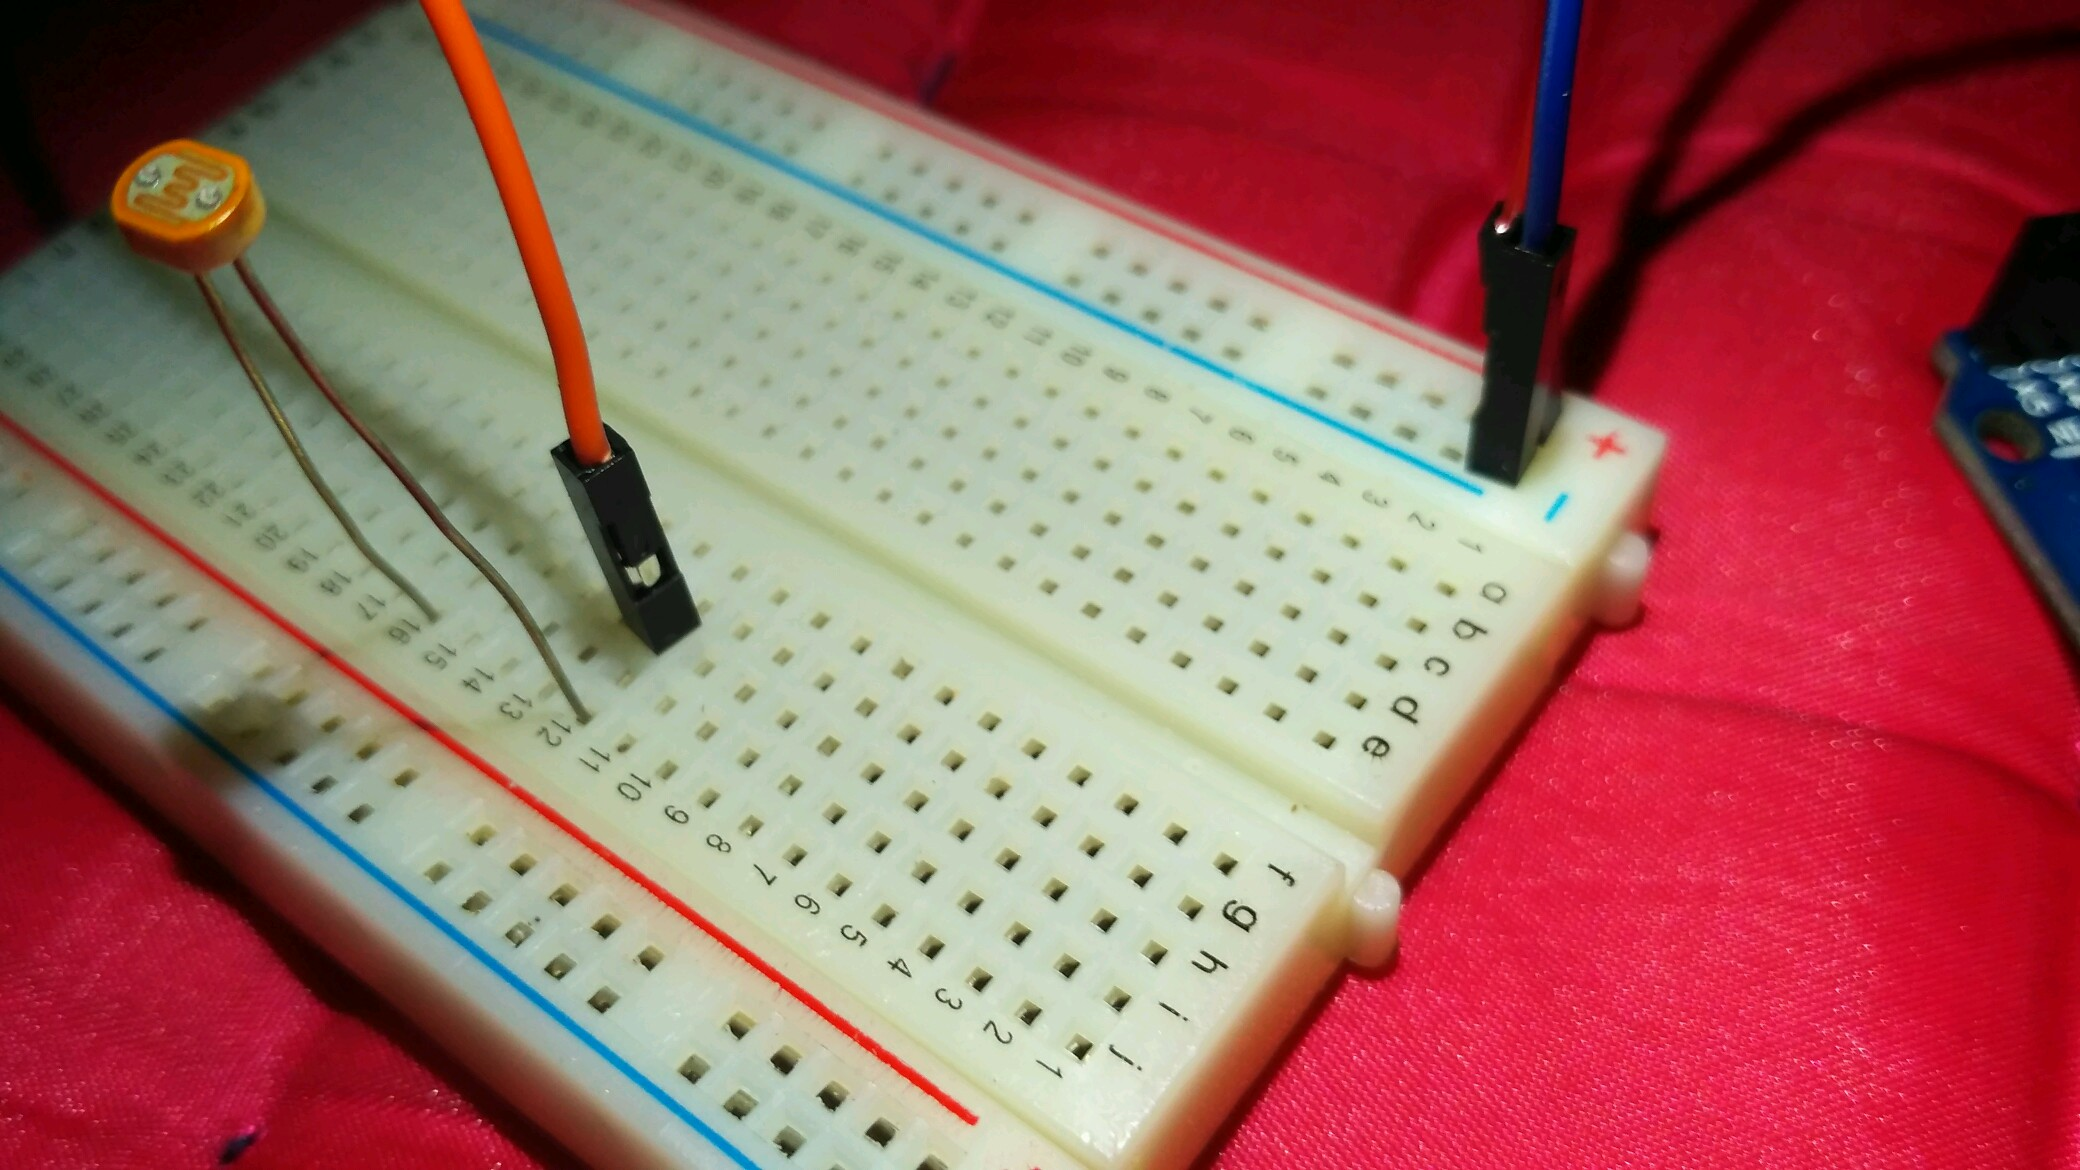
\includegraphics[width=0.9\textwidth]{figures/6.jpg}}
	\break
	\centerline{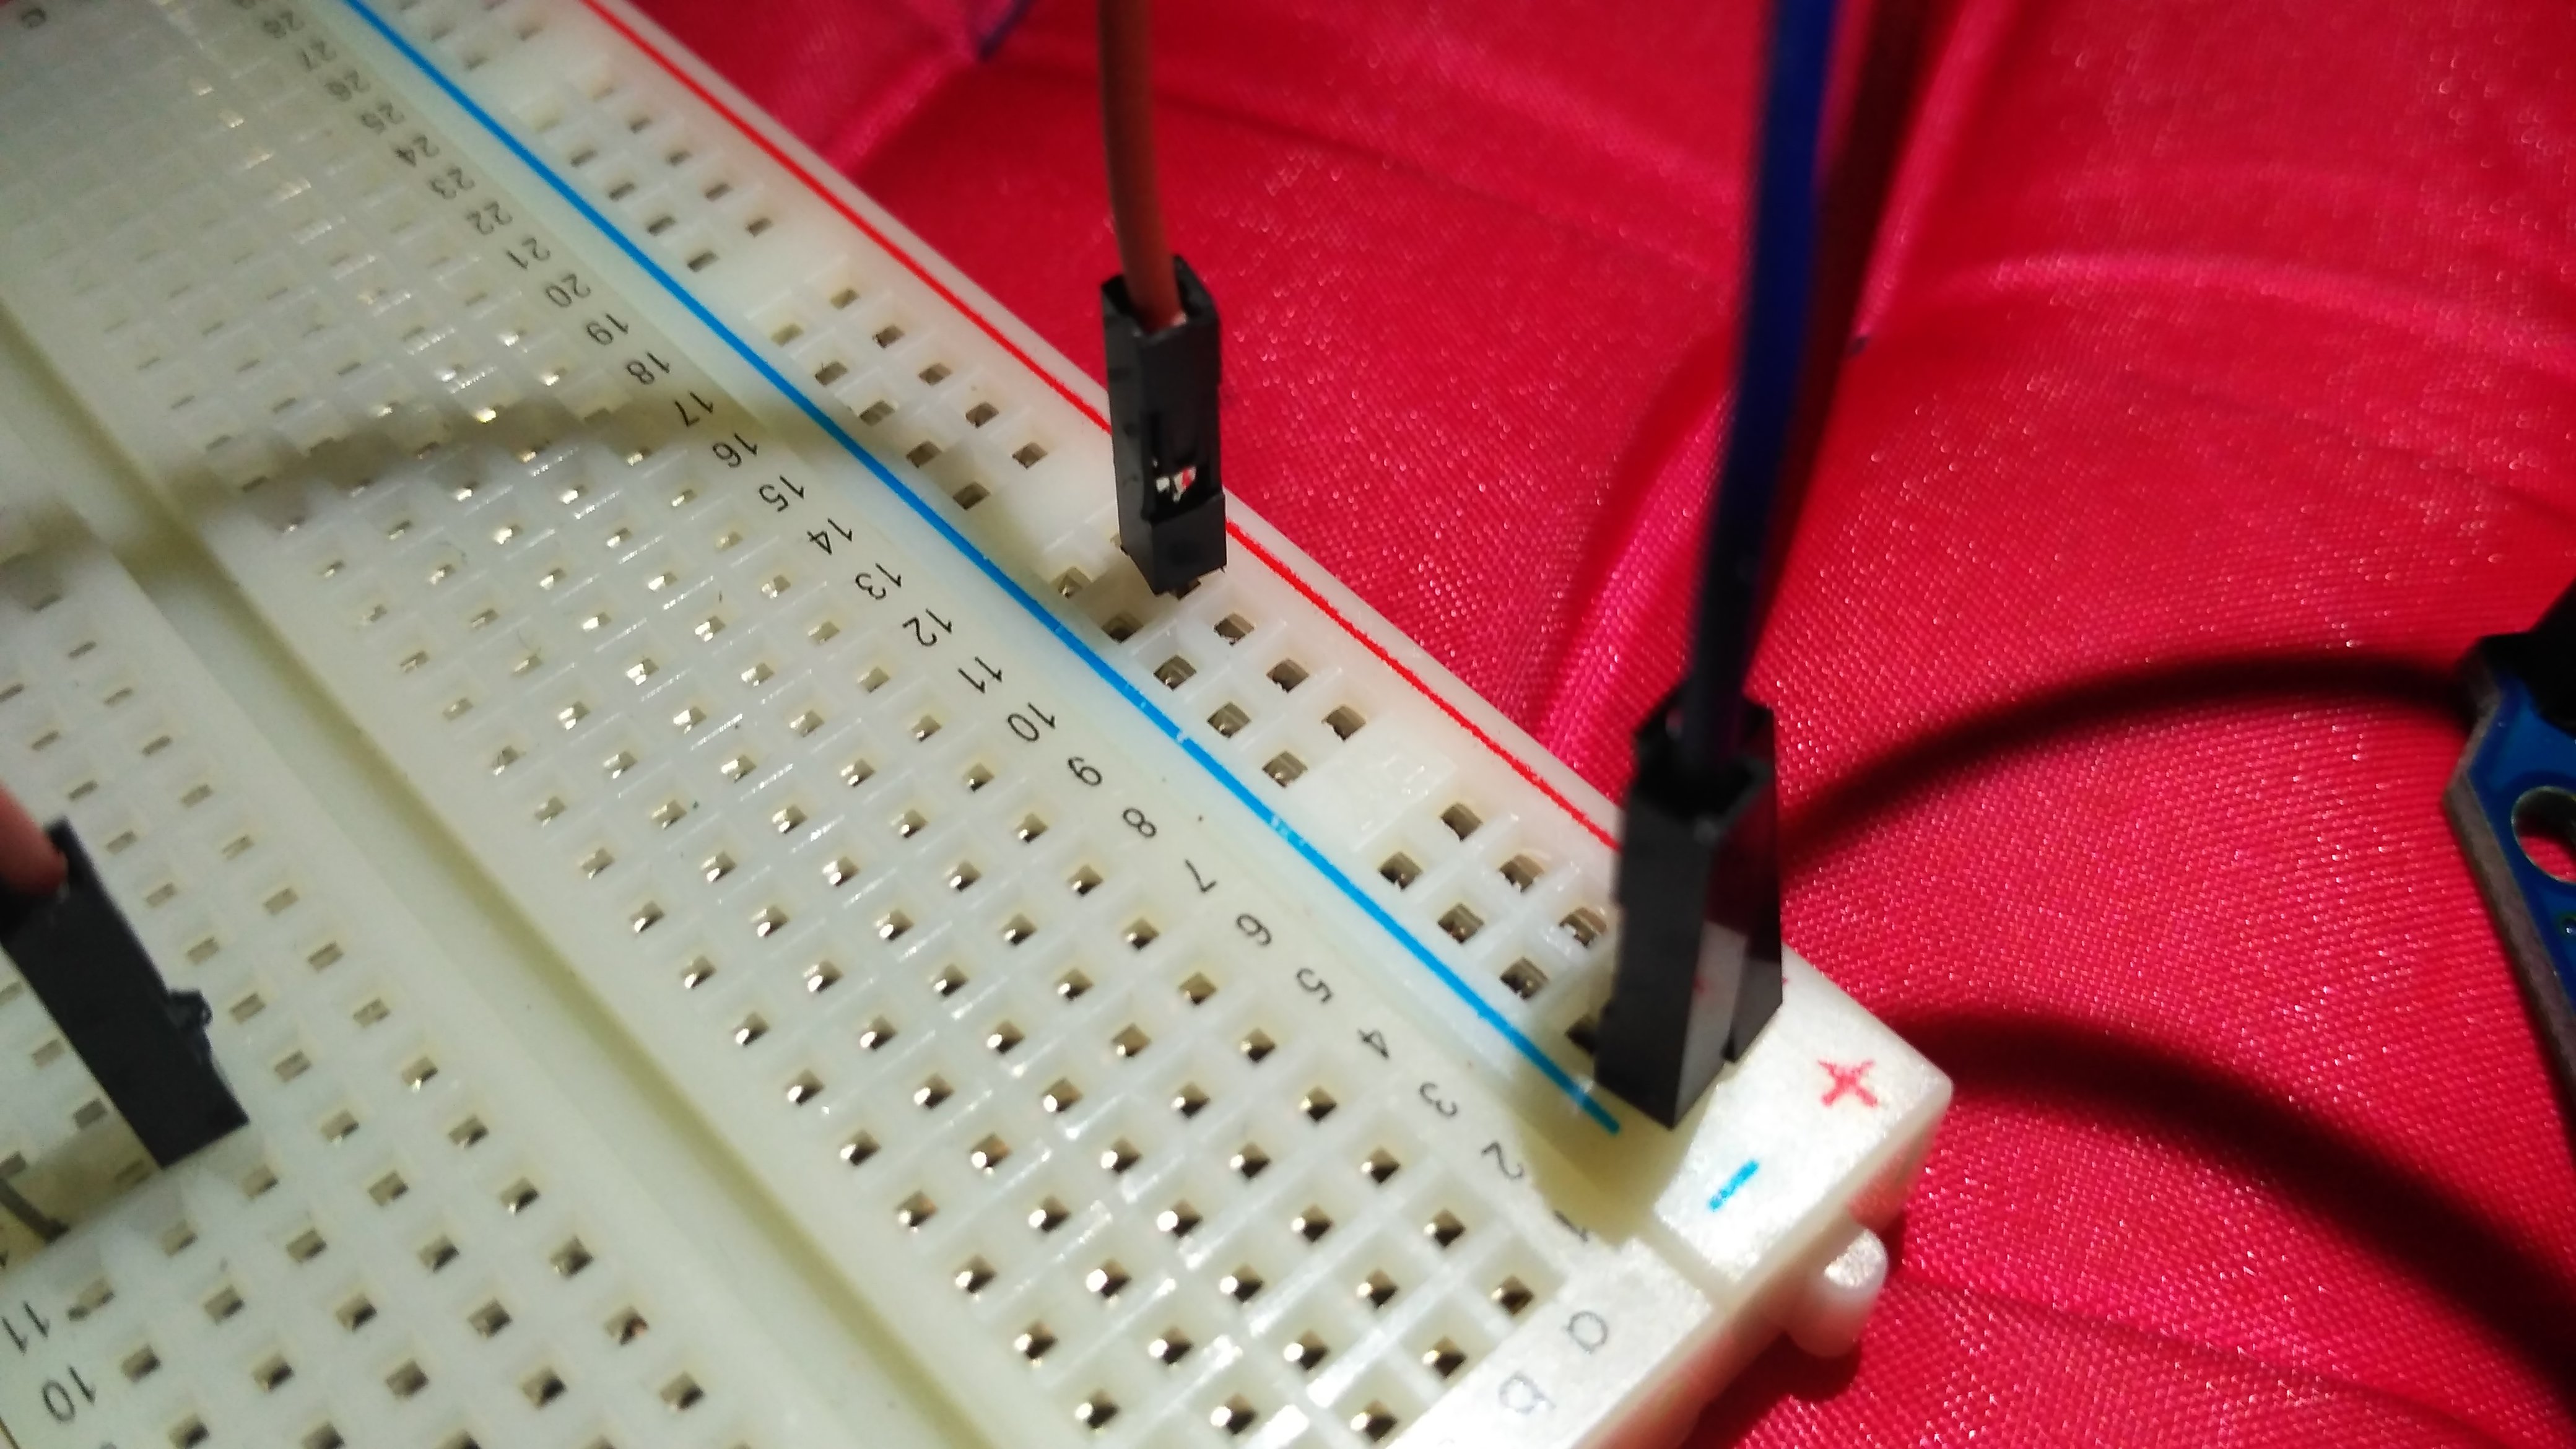
\includegraphics[width=0.9\textwidth]{figures/7.jpg}}
	\break
	\item  Kemudian pasang resistor pada g16 dan g20.
	\break
	\centerline{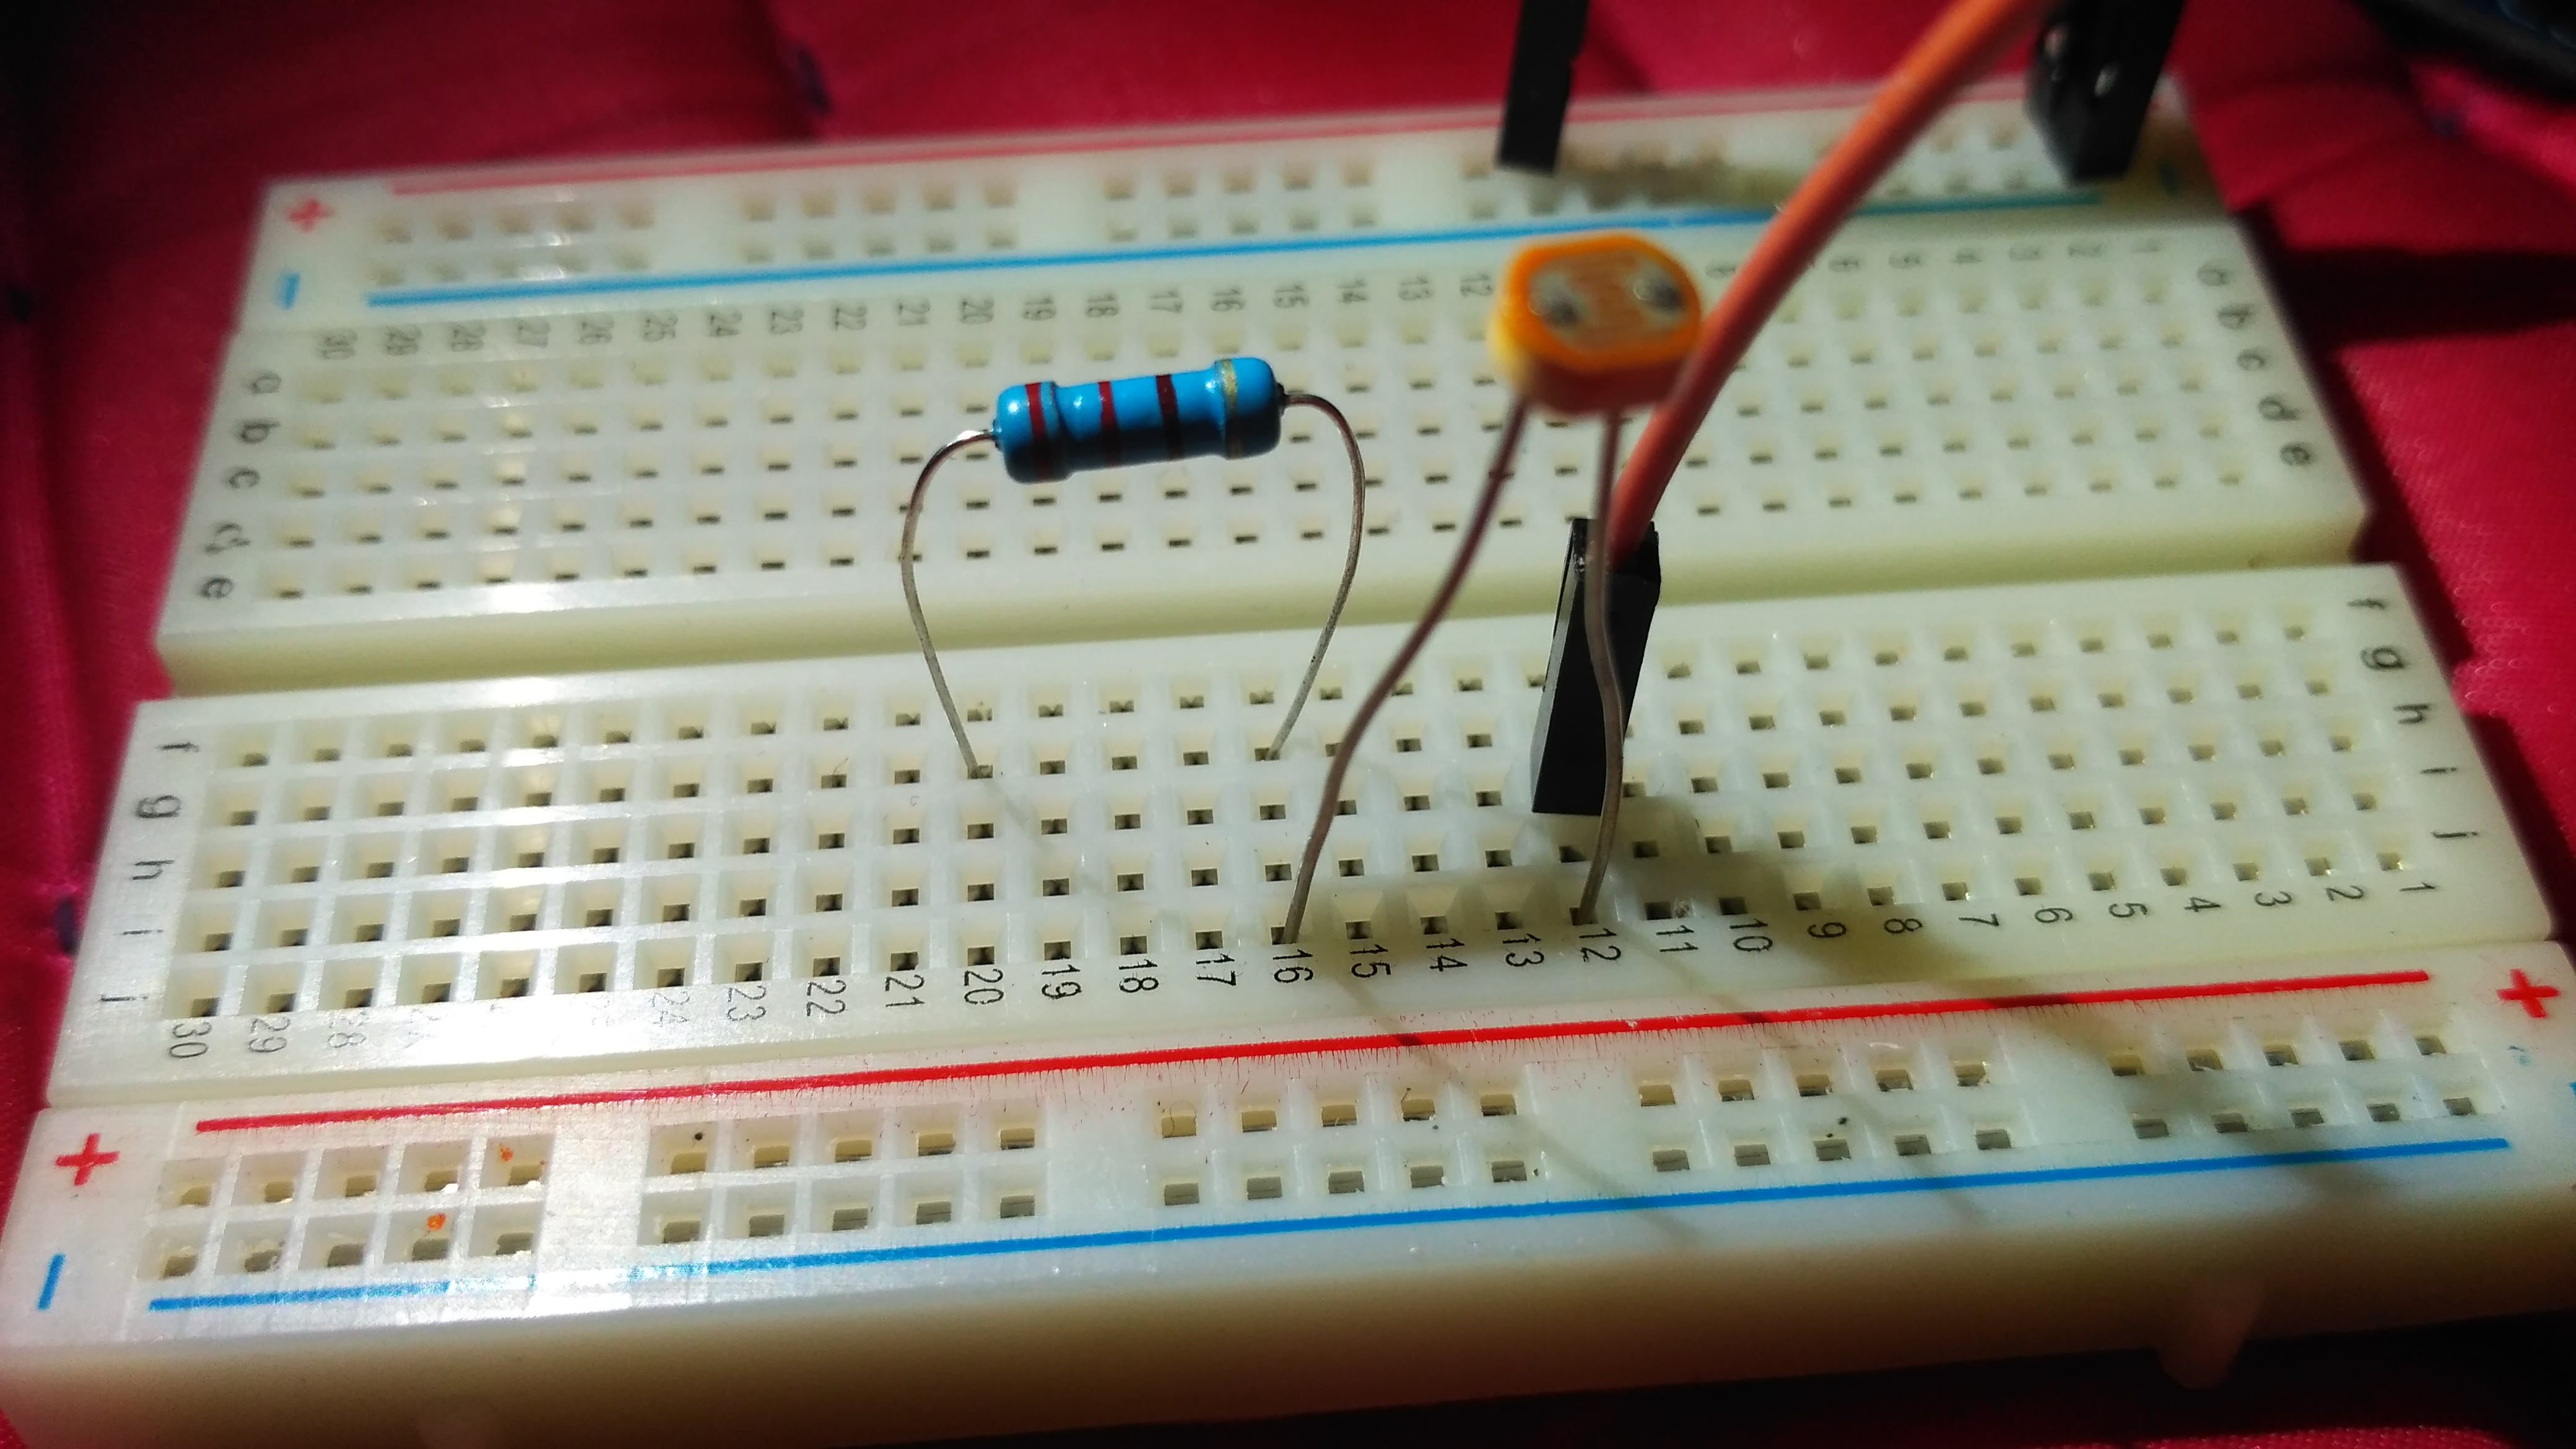
\includegraphics[width=0.9\textwidth]{figures/8.jpg}}
	\item pasangkan kabel hijau pada bredboard -20 dan ke f20.
	\break
	\centerline{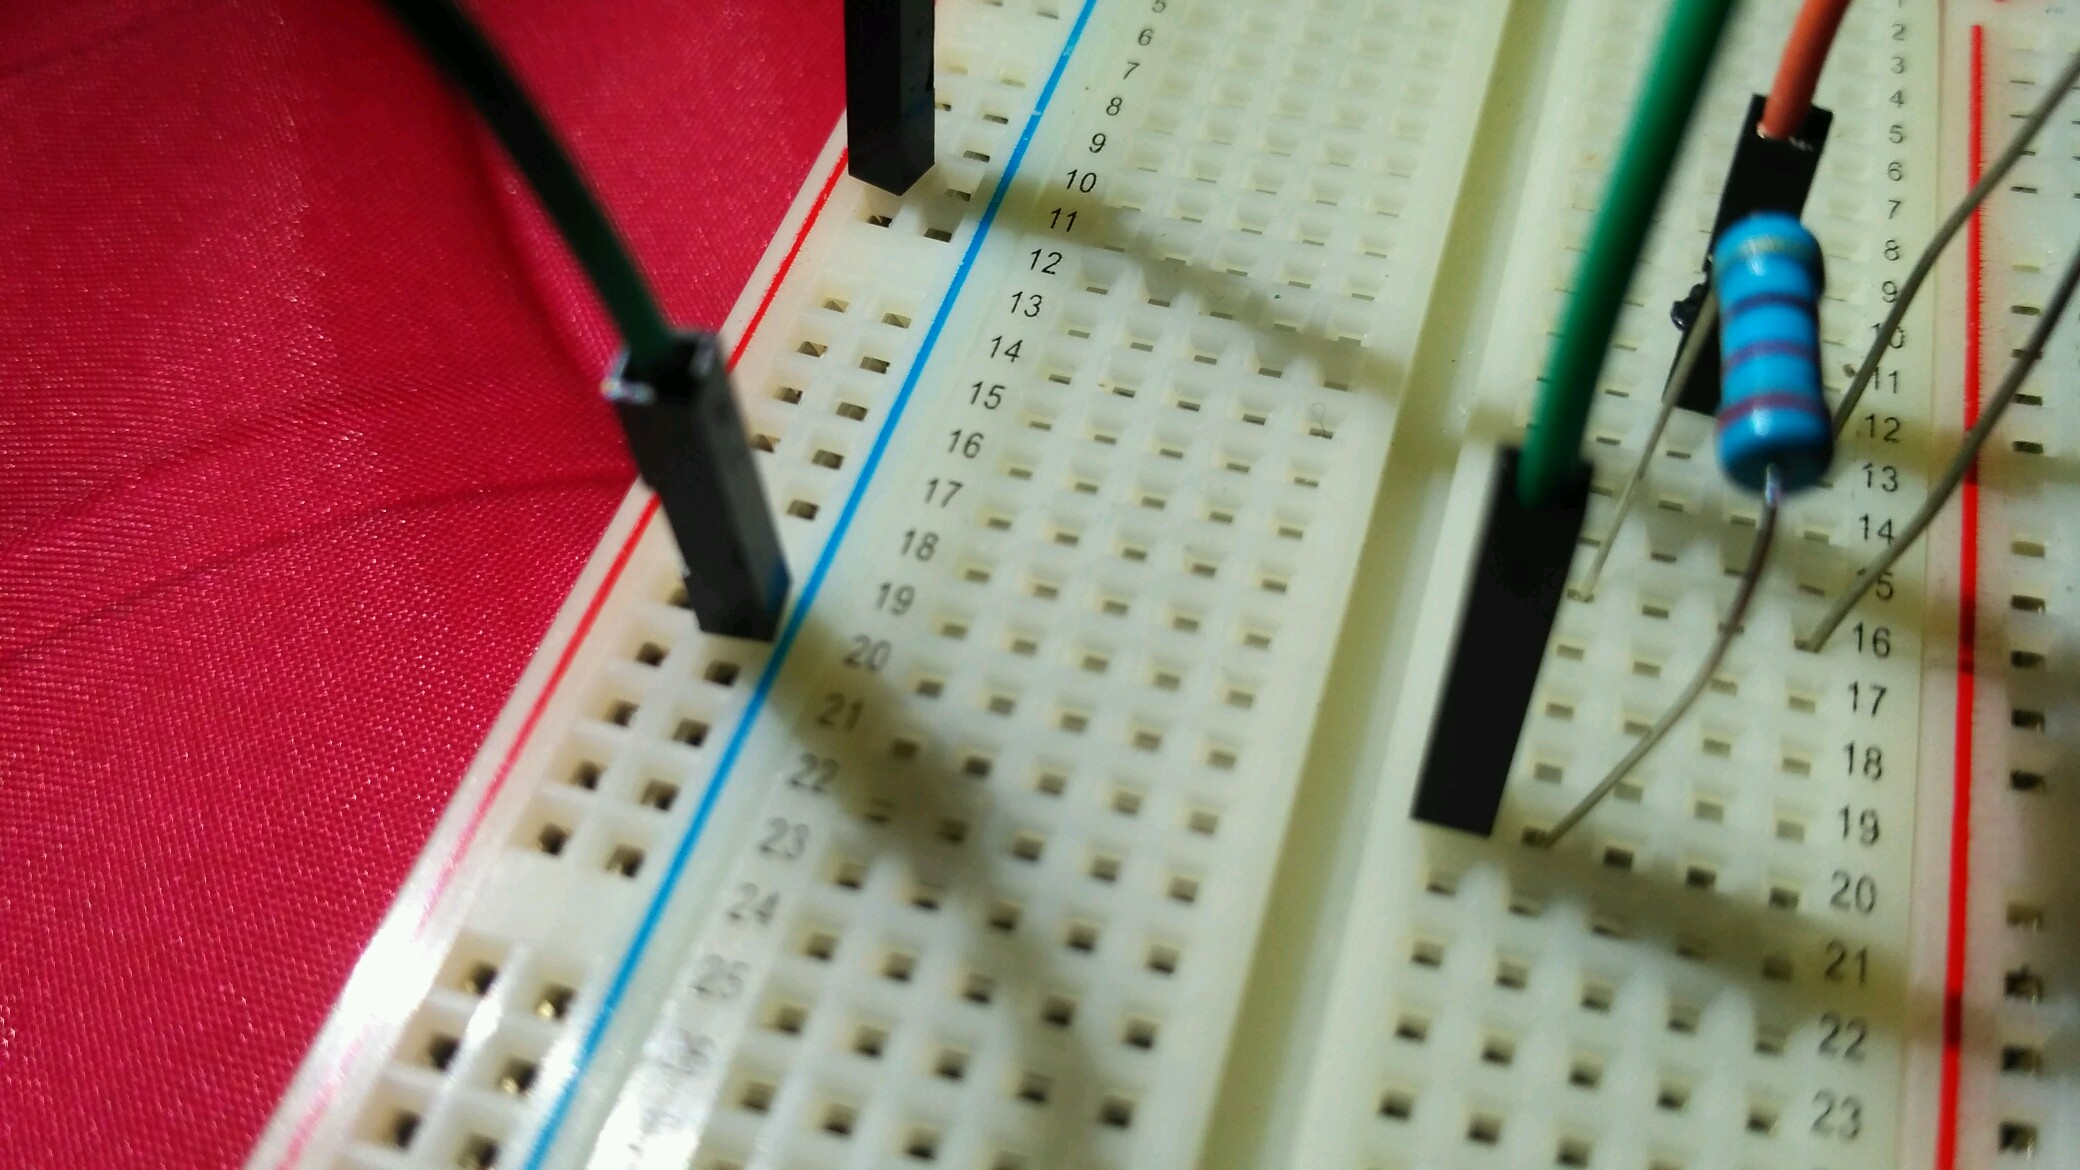
\includegraphics[width=0.9\textwidth]{figures/9.jpg}}
	\break
	\item pasang kabel kuning 1 ke bredboard f16 dan ke arduino analog in A2.
	\break
	\centerline{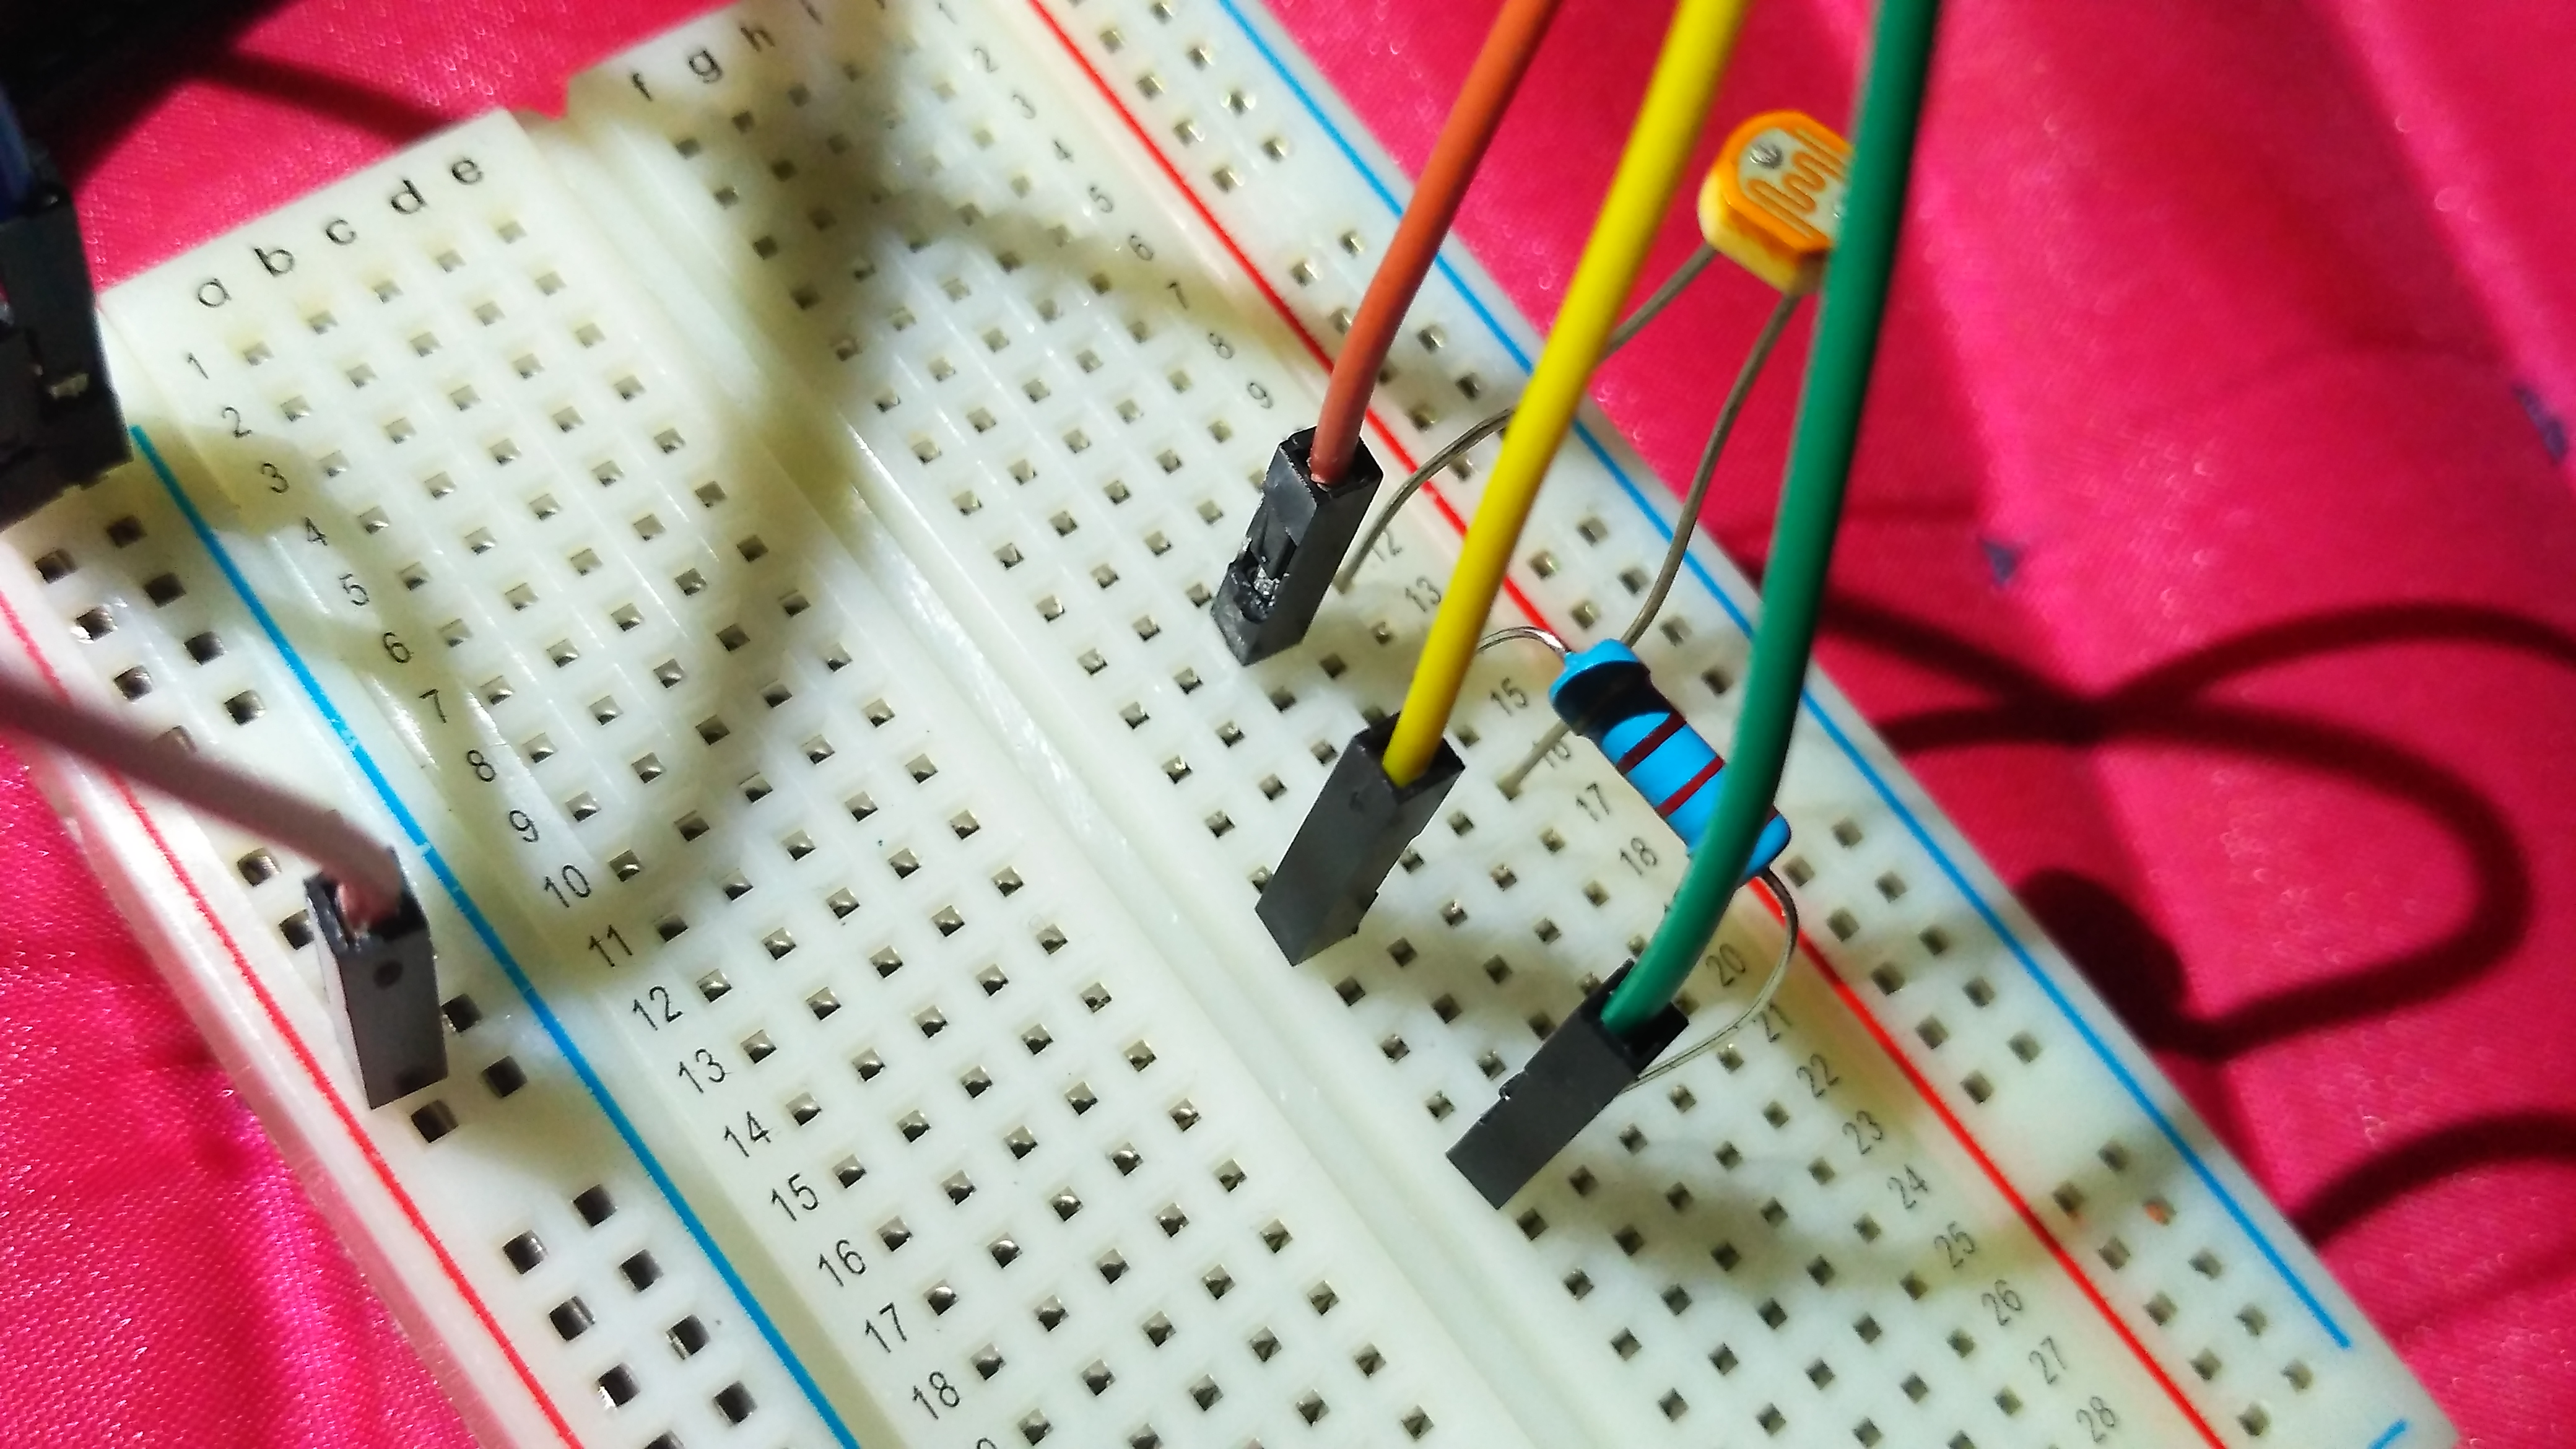
\includegraphics[width=0.9\textwidth]{figures/10.jpg}}
	\break
	\centerline{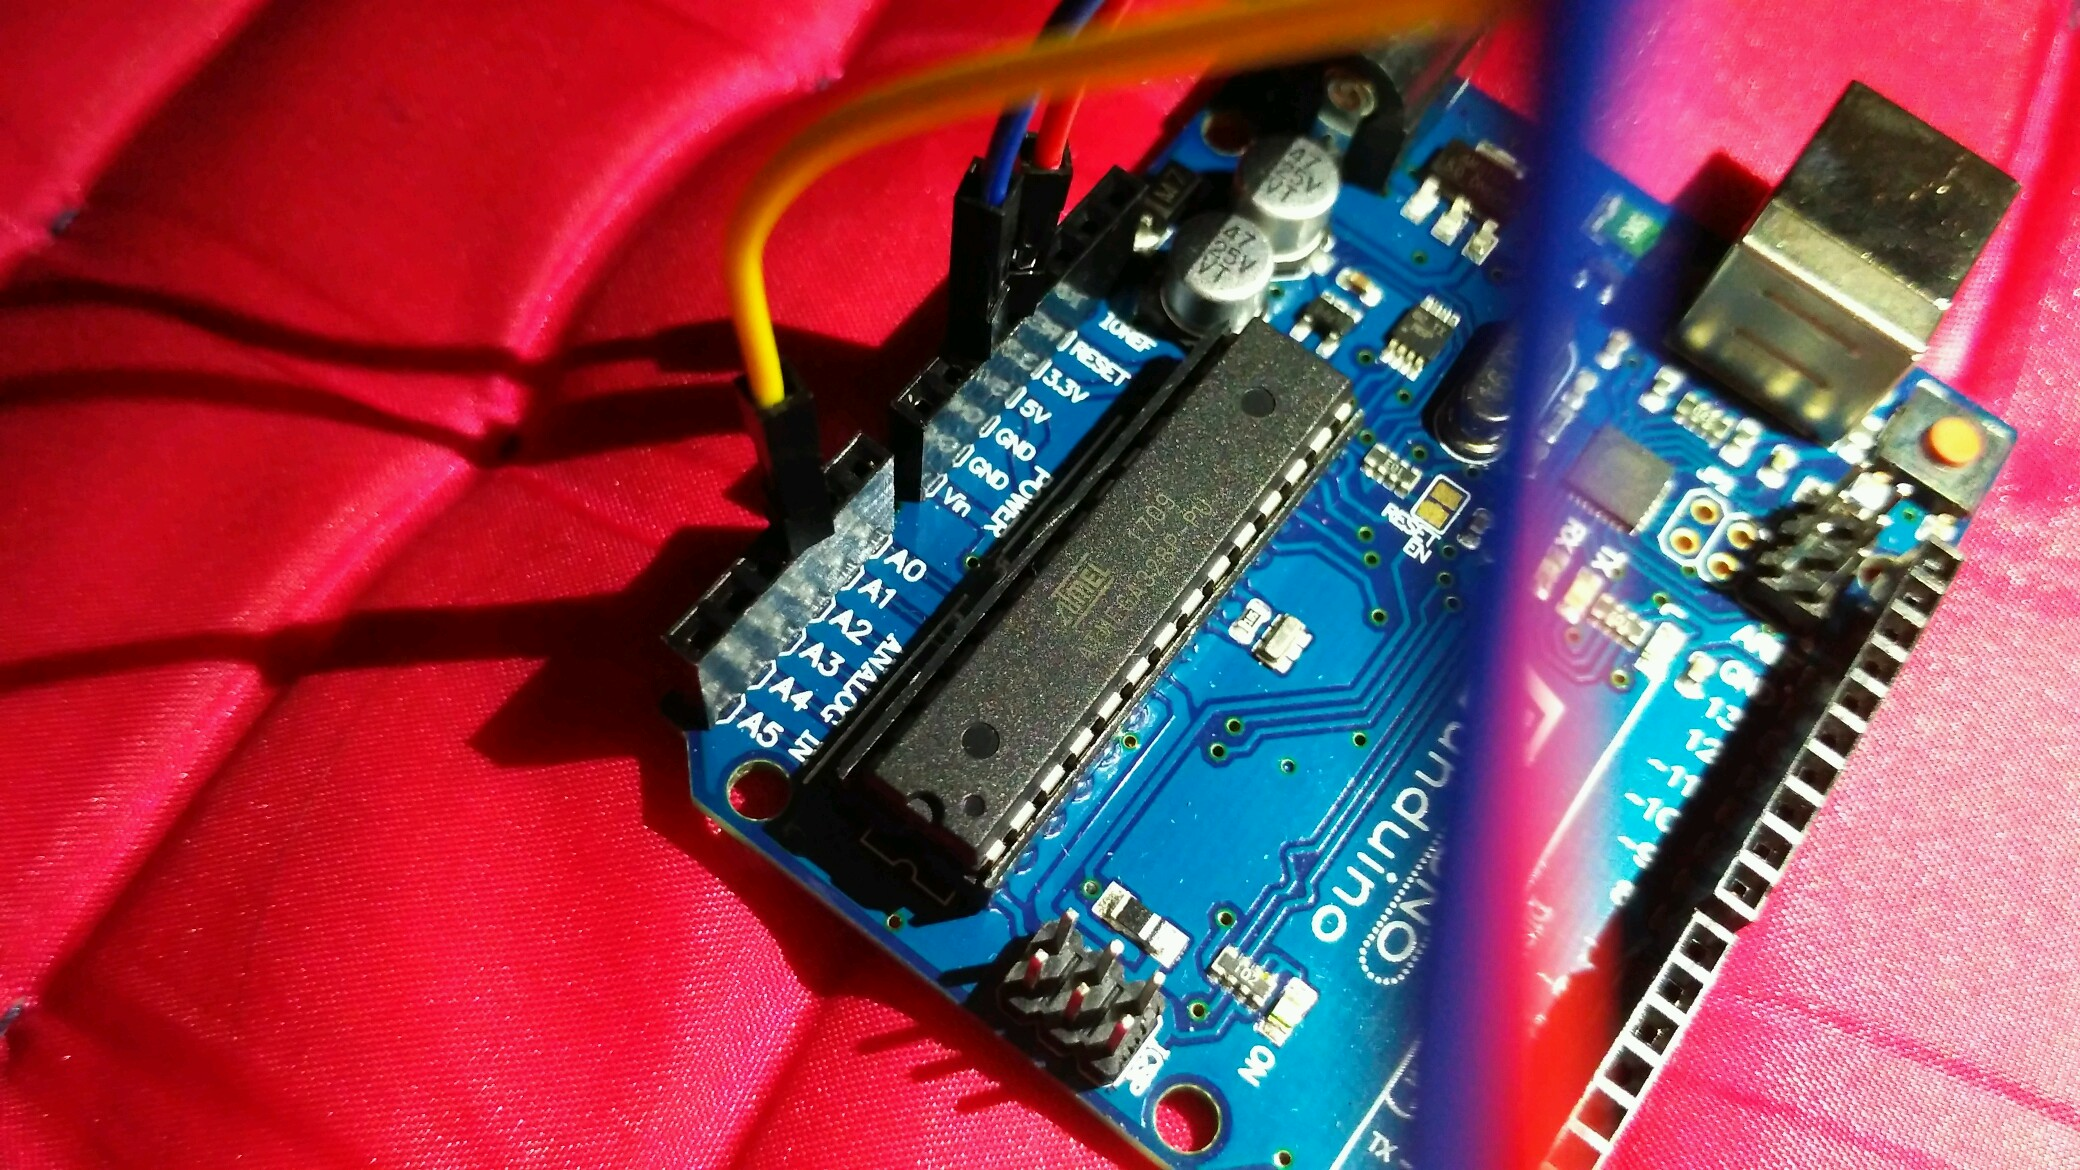
\includegraphics[width=0.9\textwidth]{figures/11.jpg}}
	\break
	\item pasang LED positif(panjang) di j1 dan negatif(pendek) di j3.
	\break
	\centerline{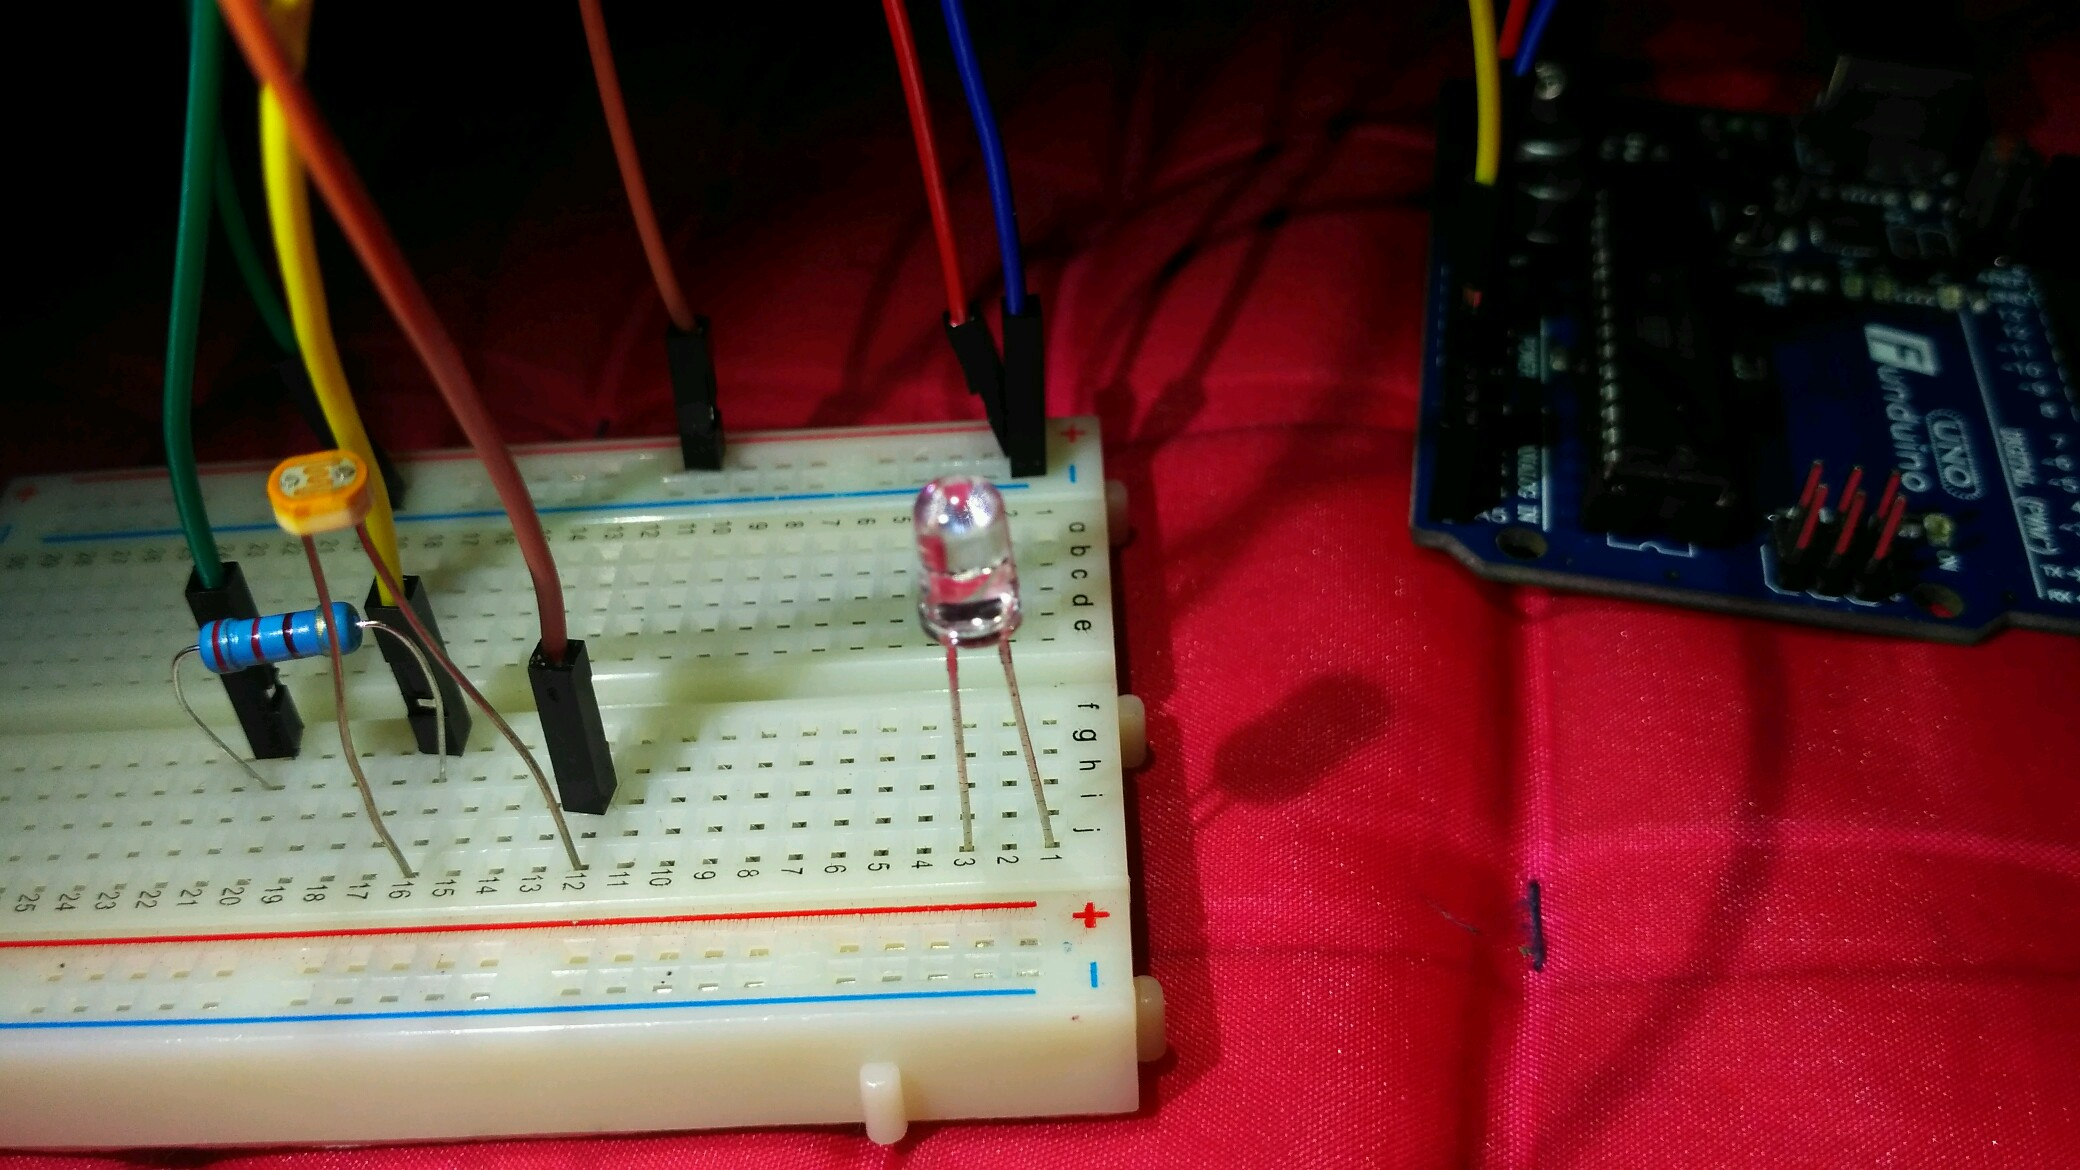
\includegraphics[width=0.9\textwidth]{figures/12.jpg}}
	\break
	\item pasang kabel kuning 2 ke bredboard f1 dan di arduino ke digital 13.
	\break
	\centerline{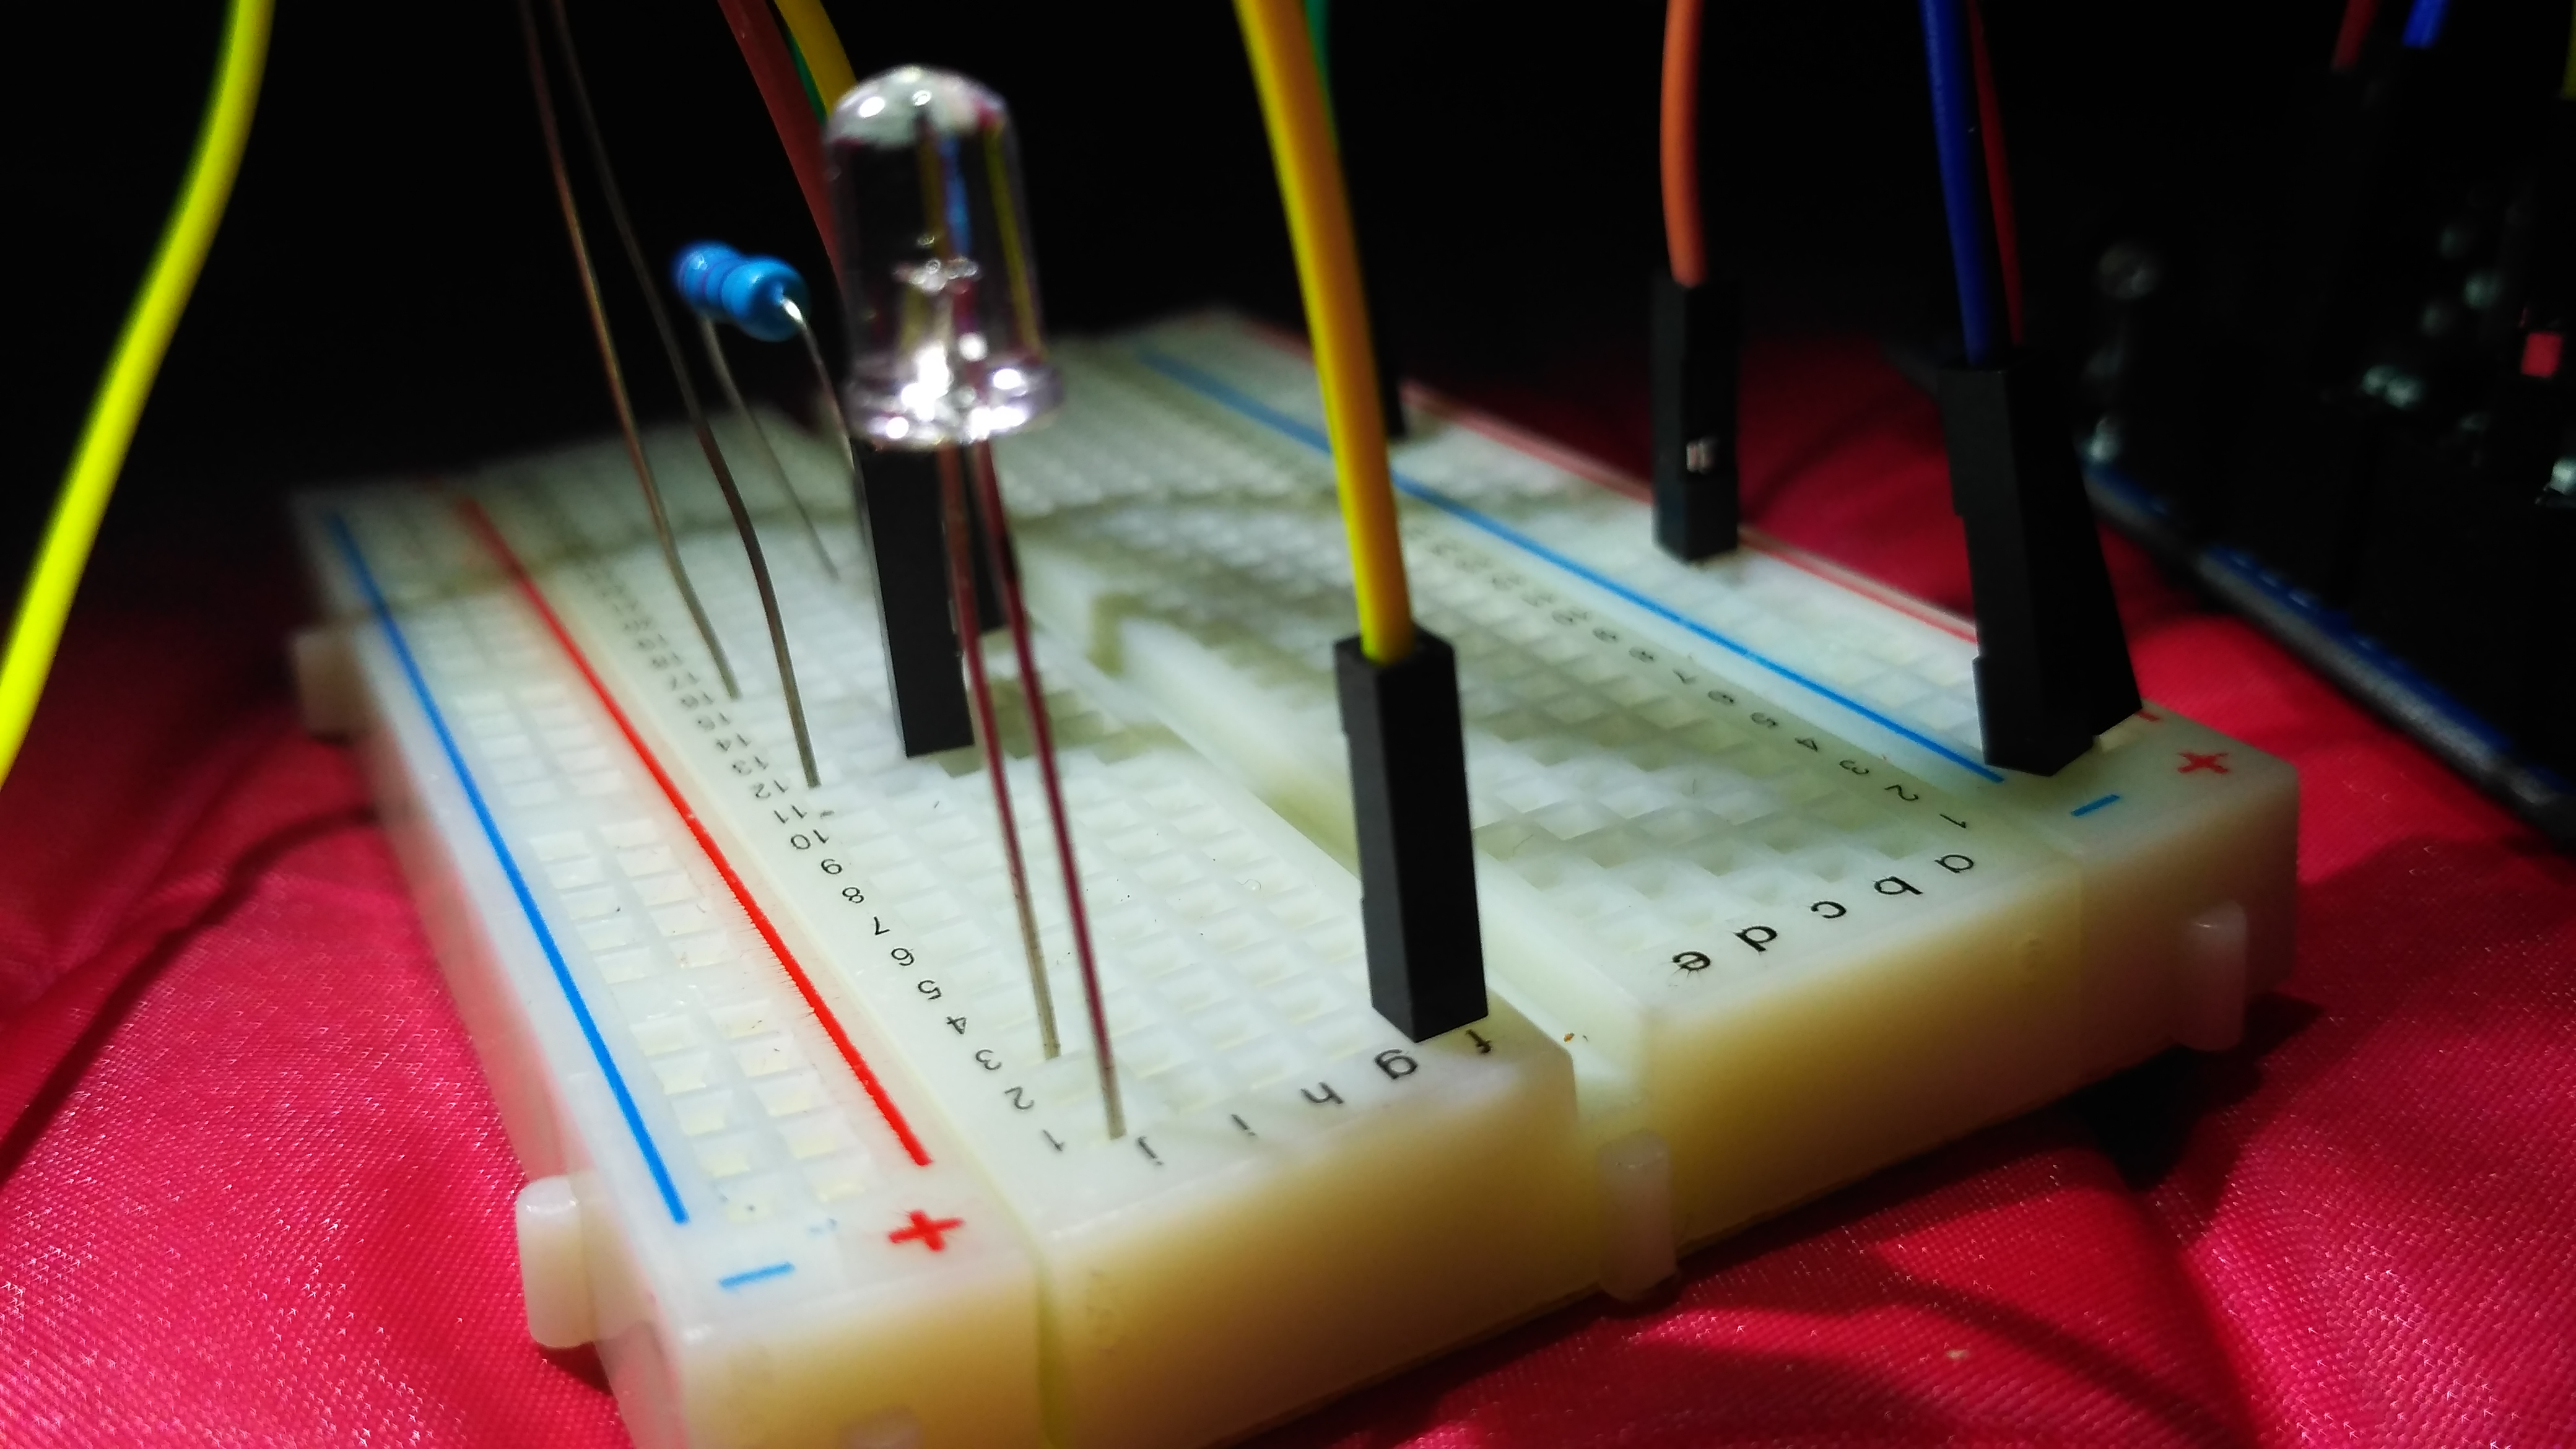
\includegraphics[width=0.9\textwidth]{figures/13.jpg}}
	\break
	\centerline{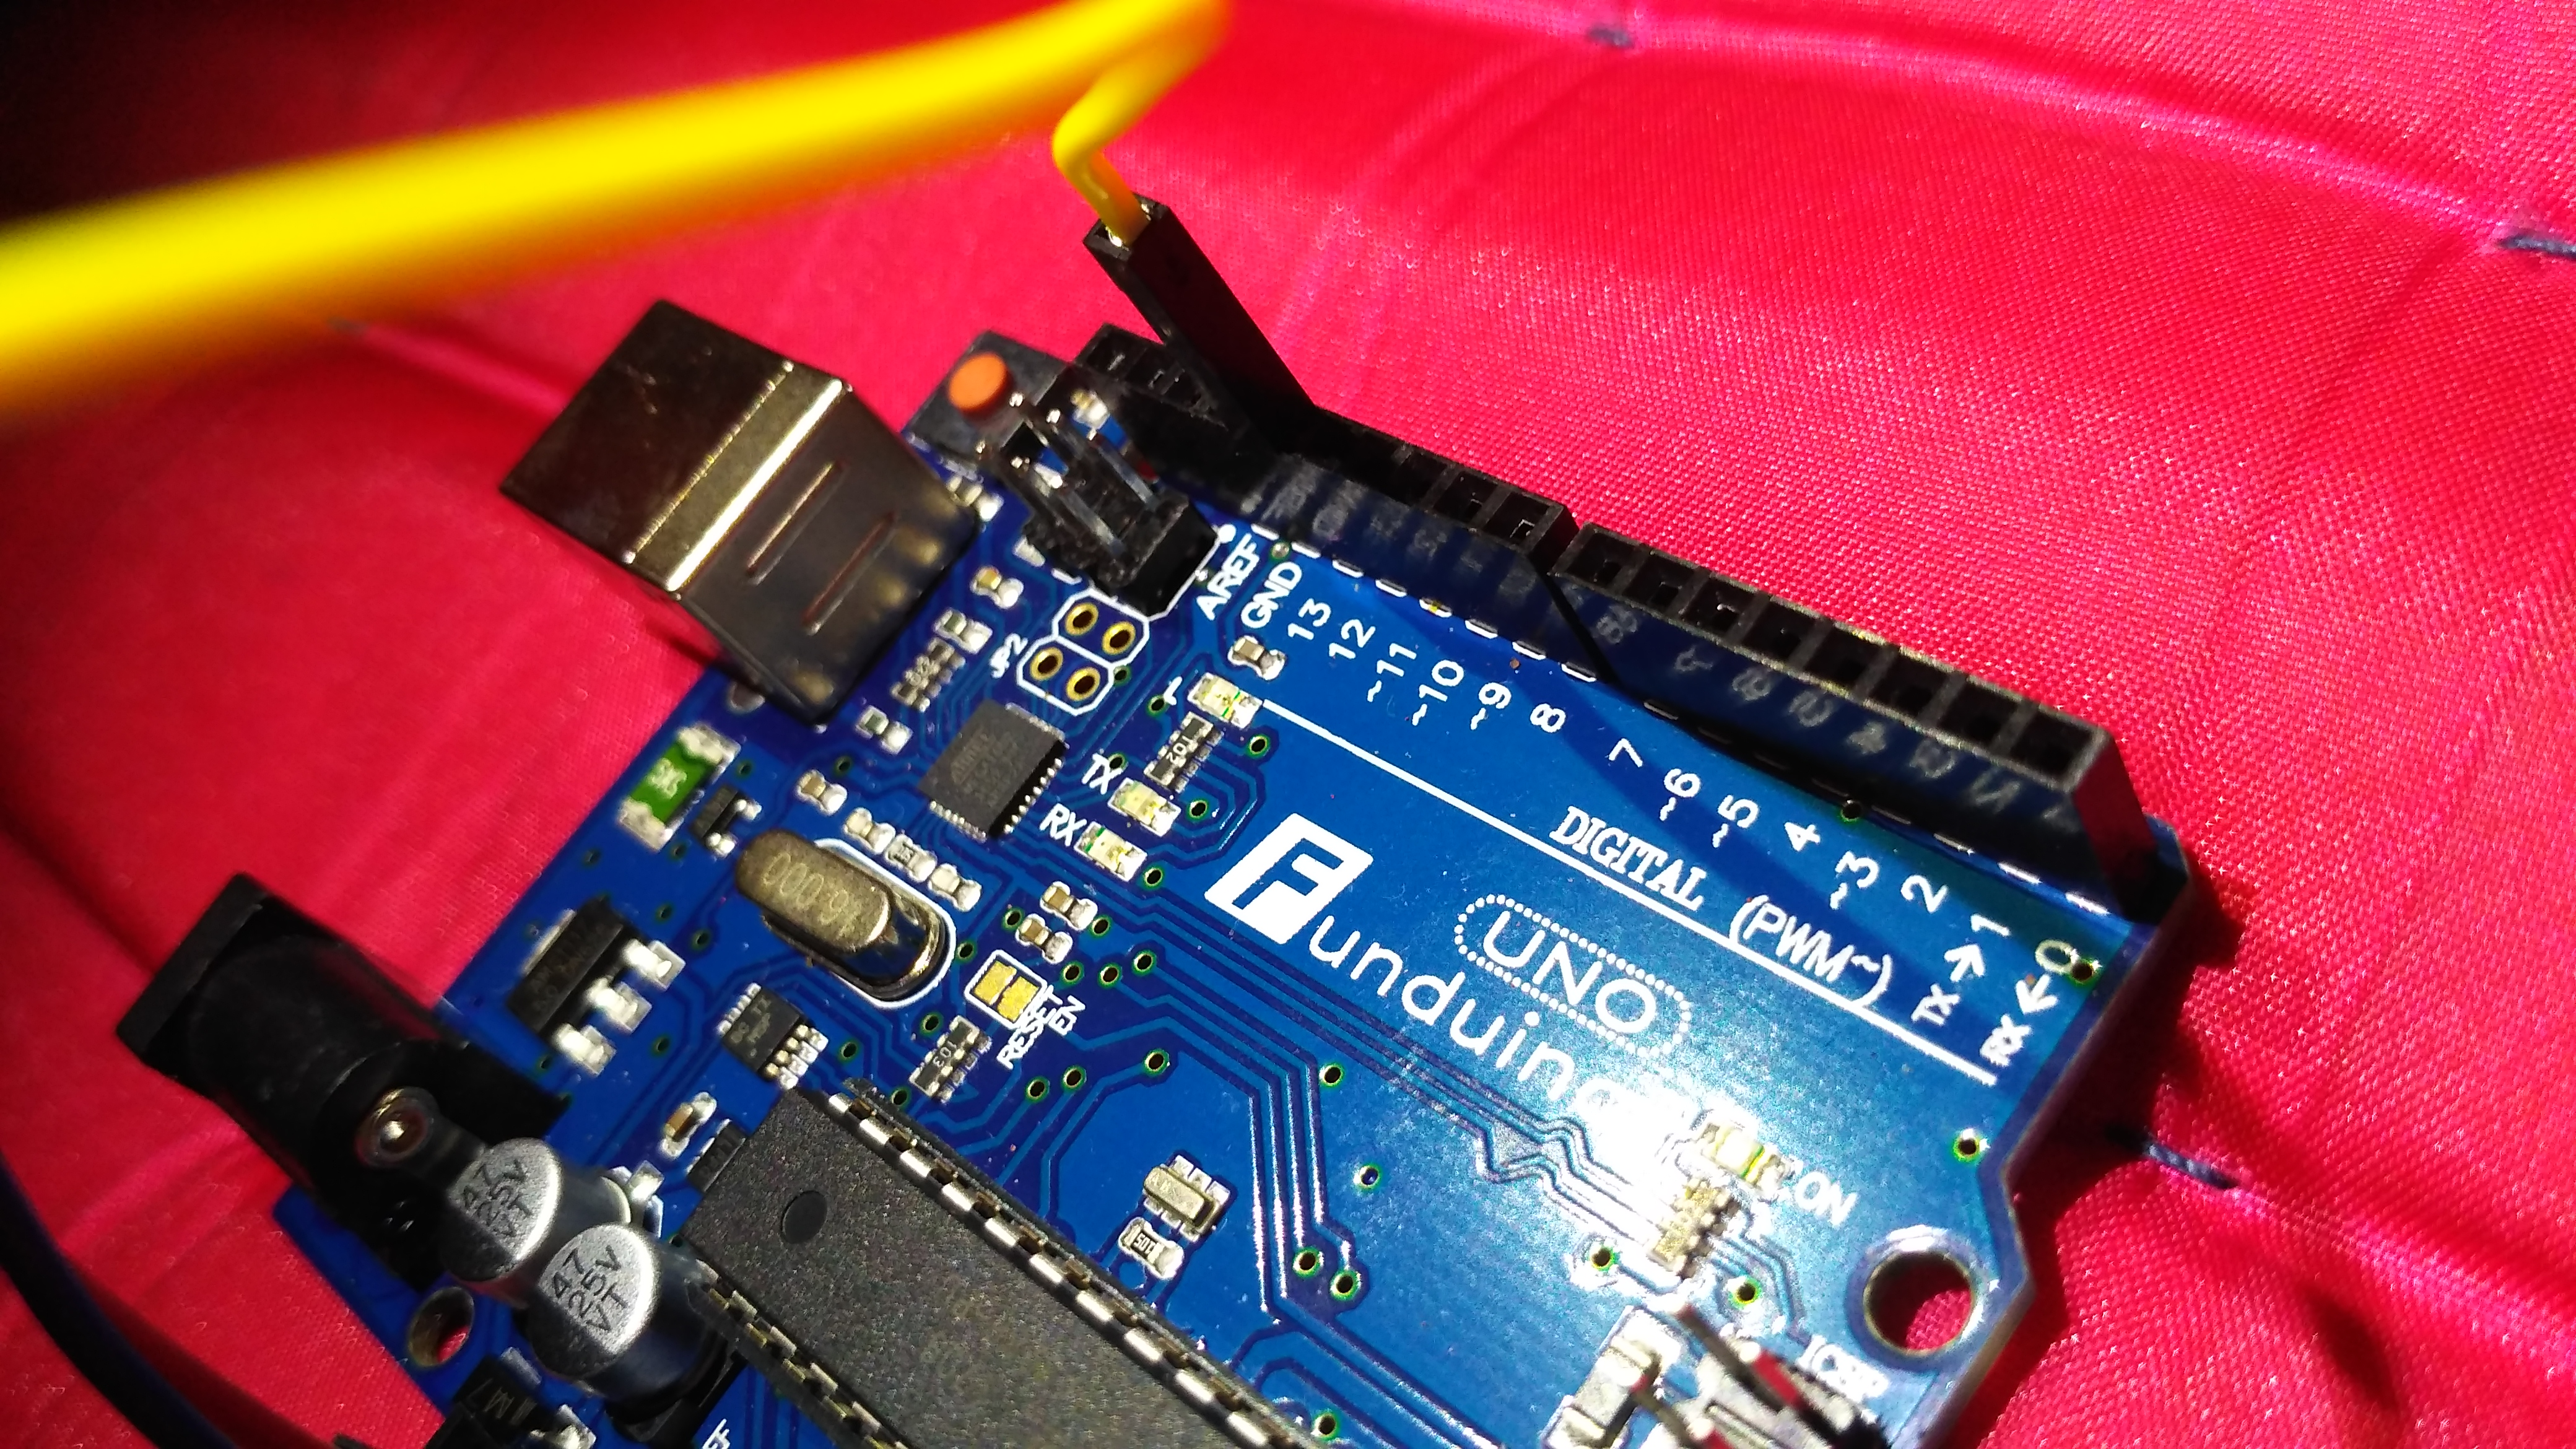
\includegraphics[width=0.9\textwidth]{figures/14.jpg}}
	\break
	\item pasang kabel orange ke bredboard f3 dan ke bredboard -6.
	\break
	\centerline{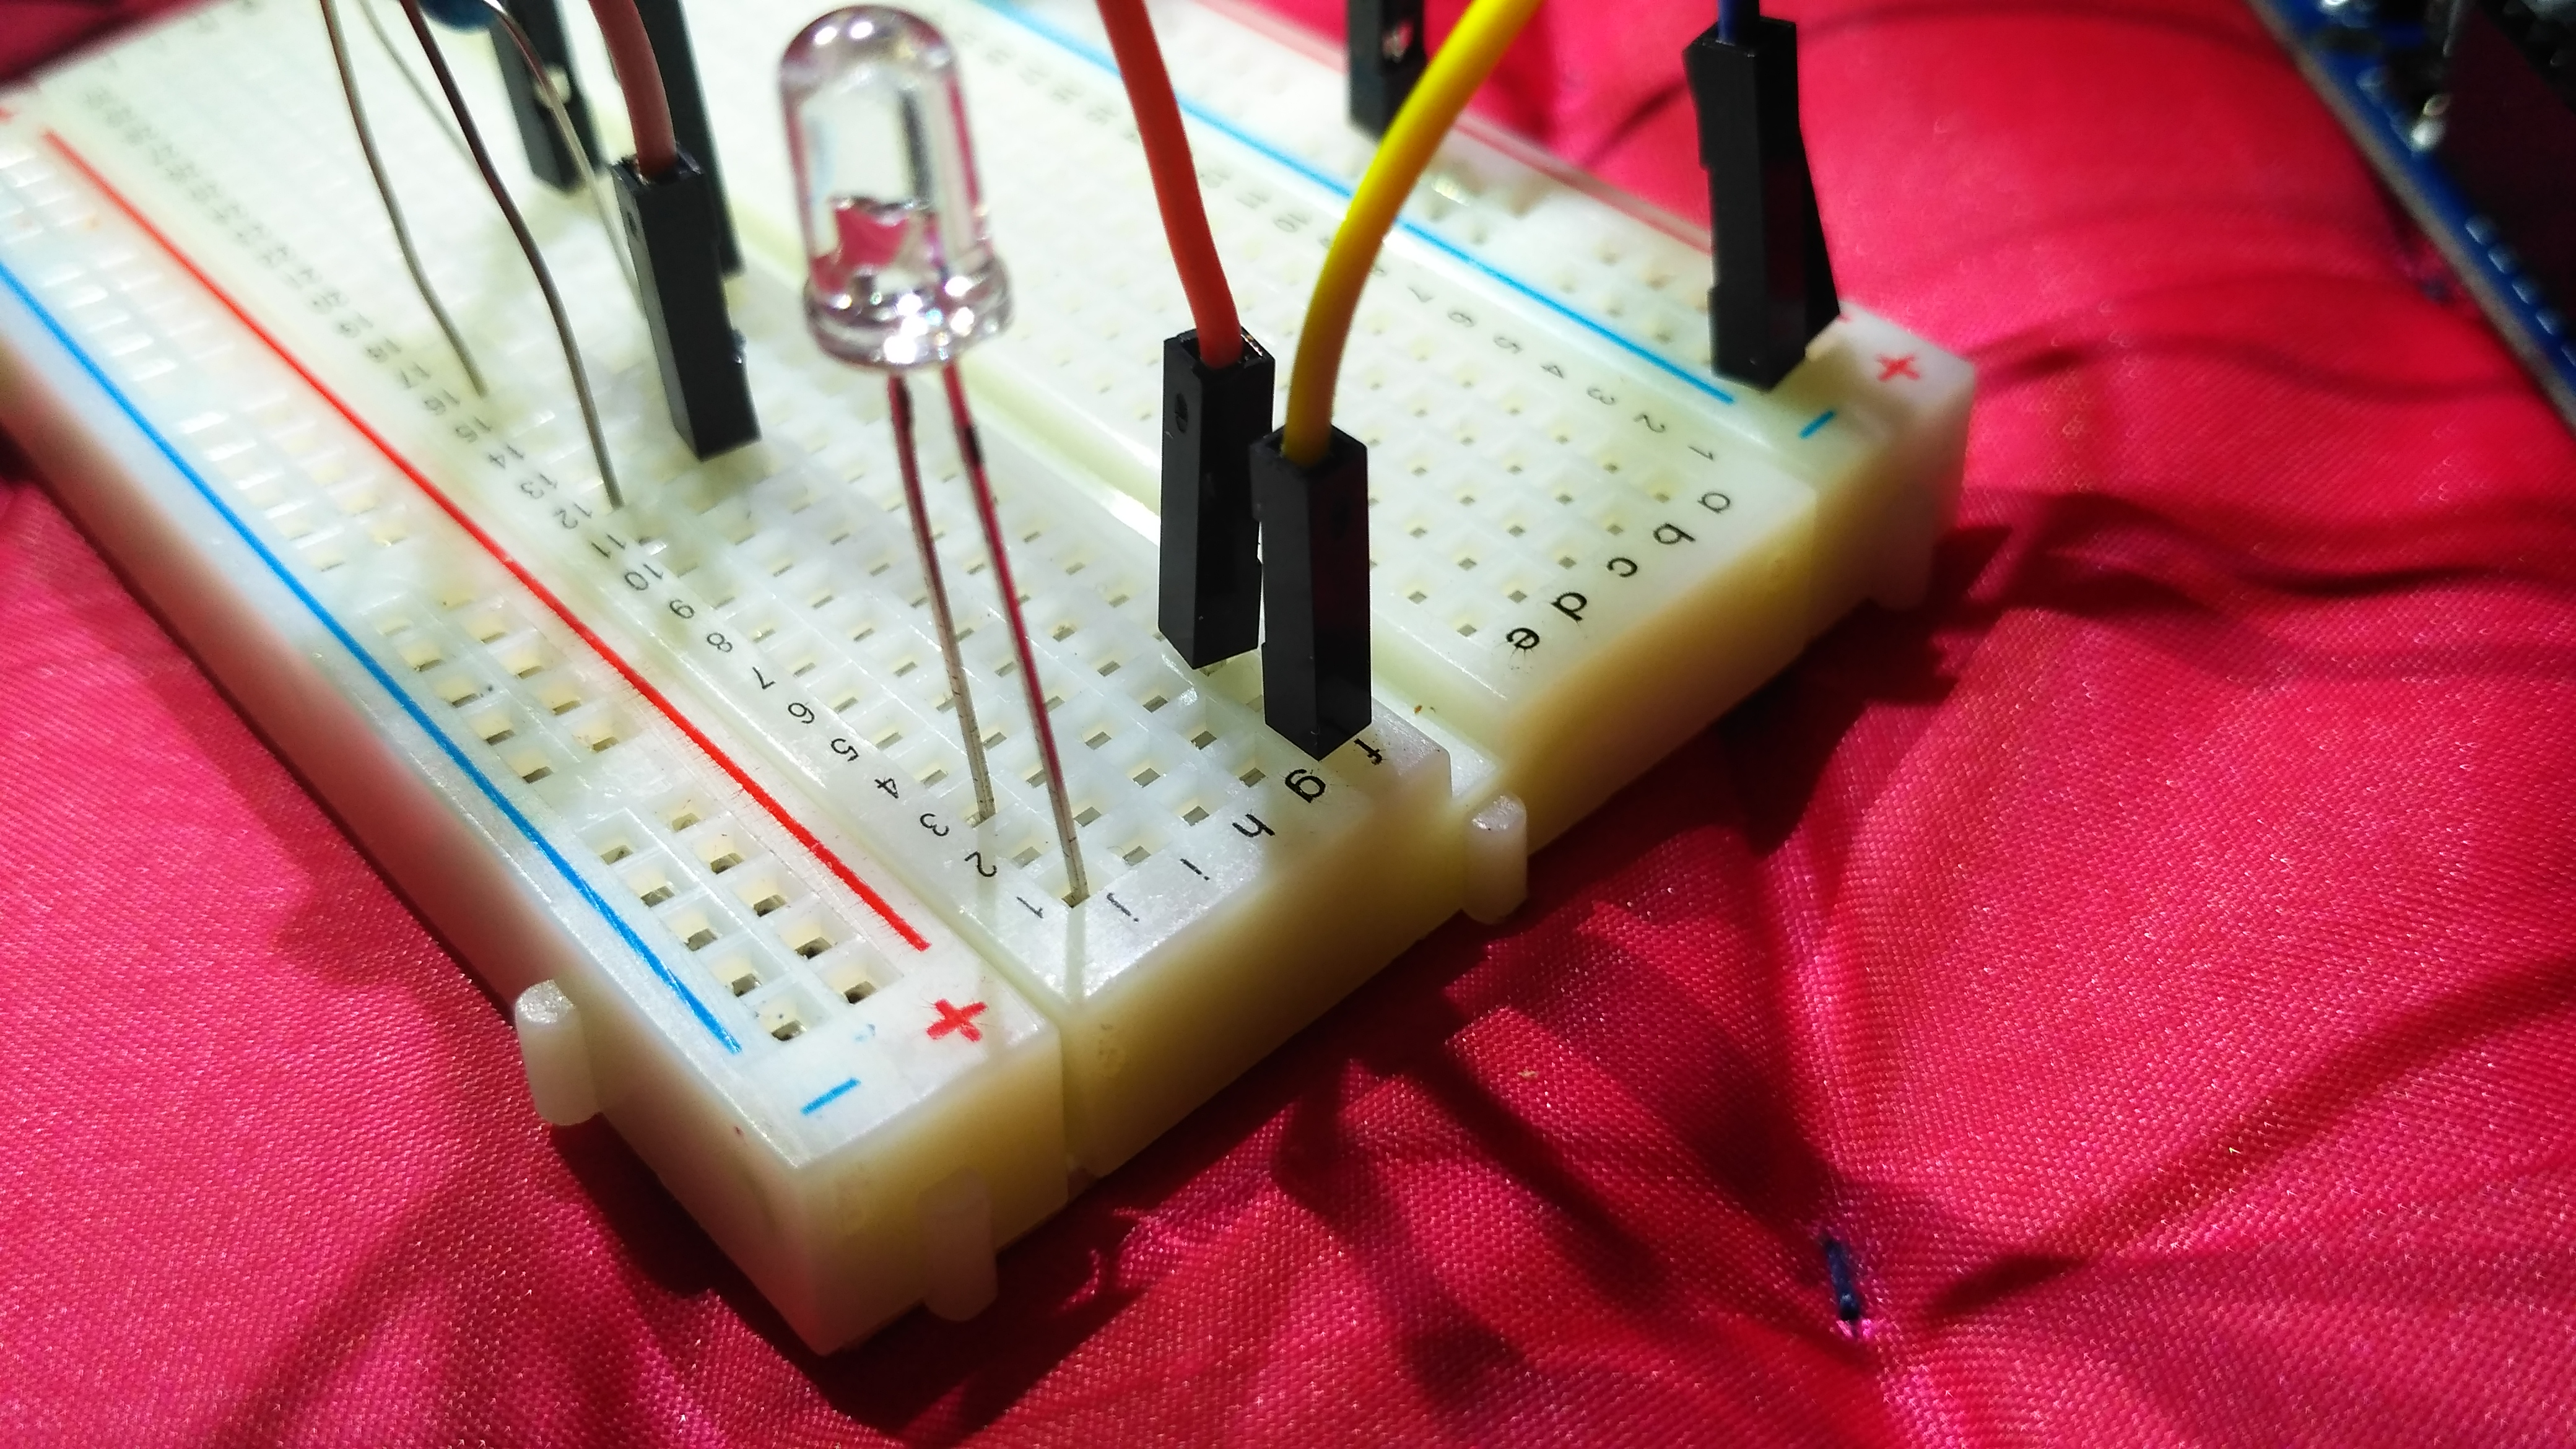
\includegraphics[width=0.9\textwidth]{figures/15.jpg}}
	\break
	\centerline{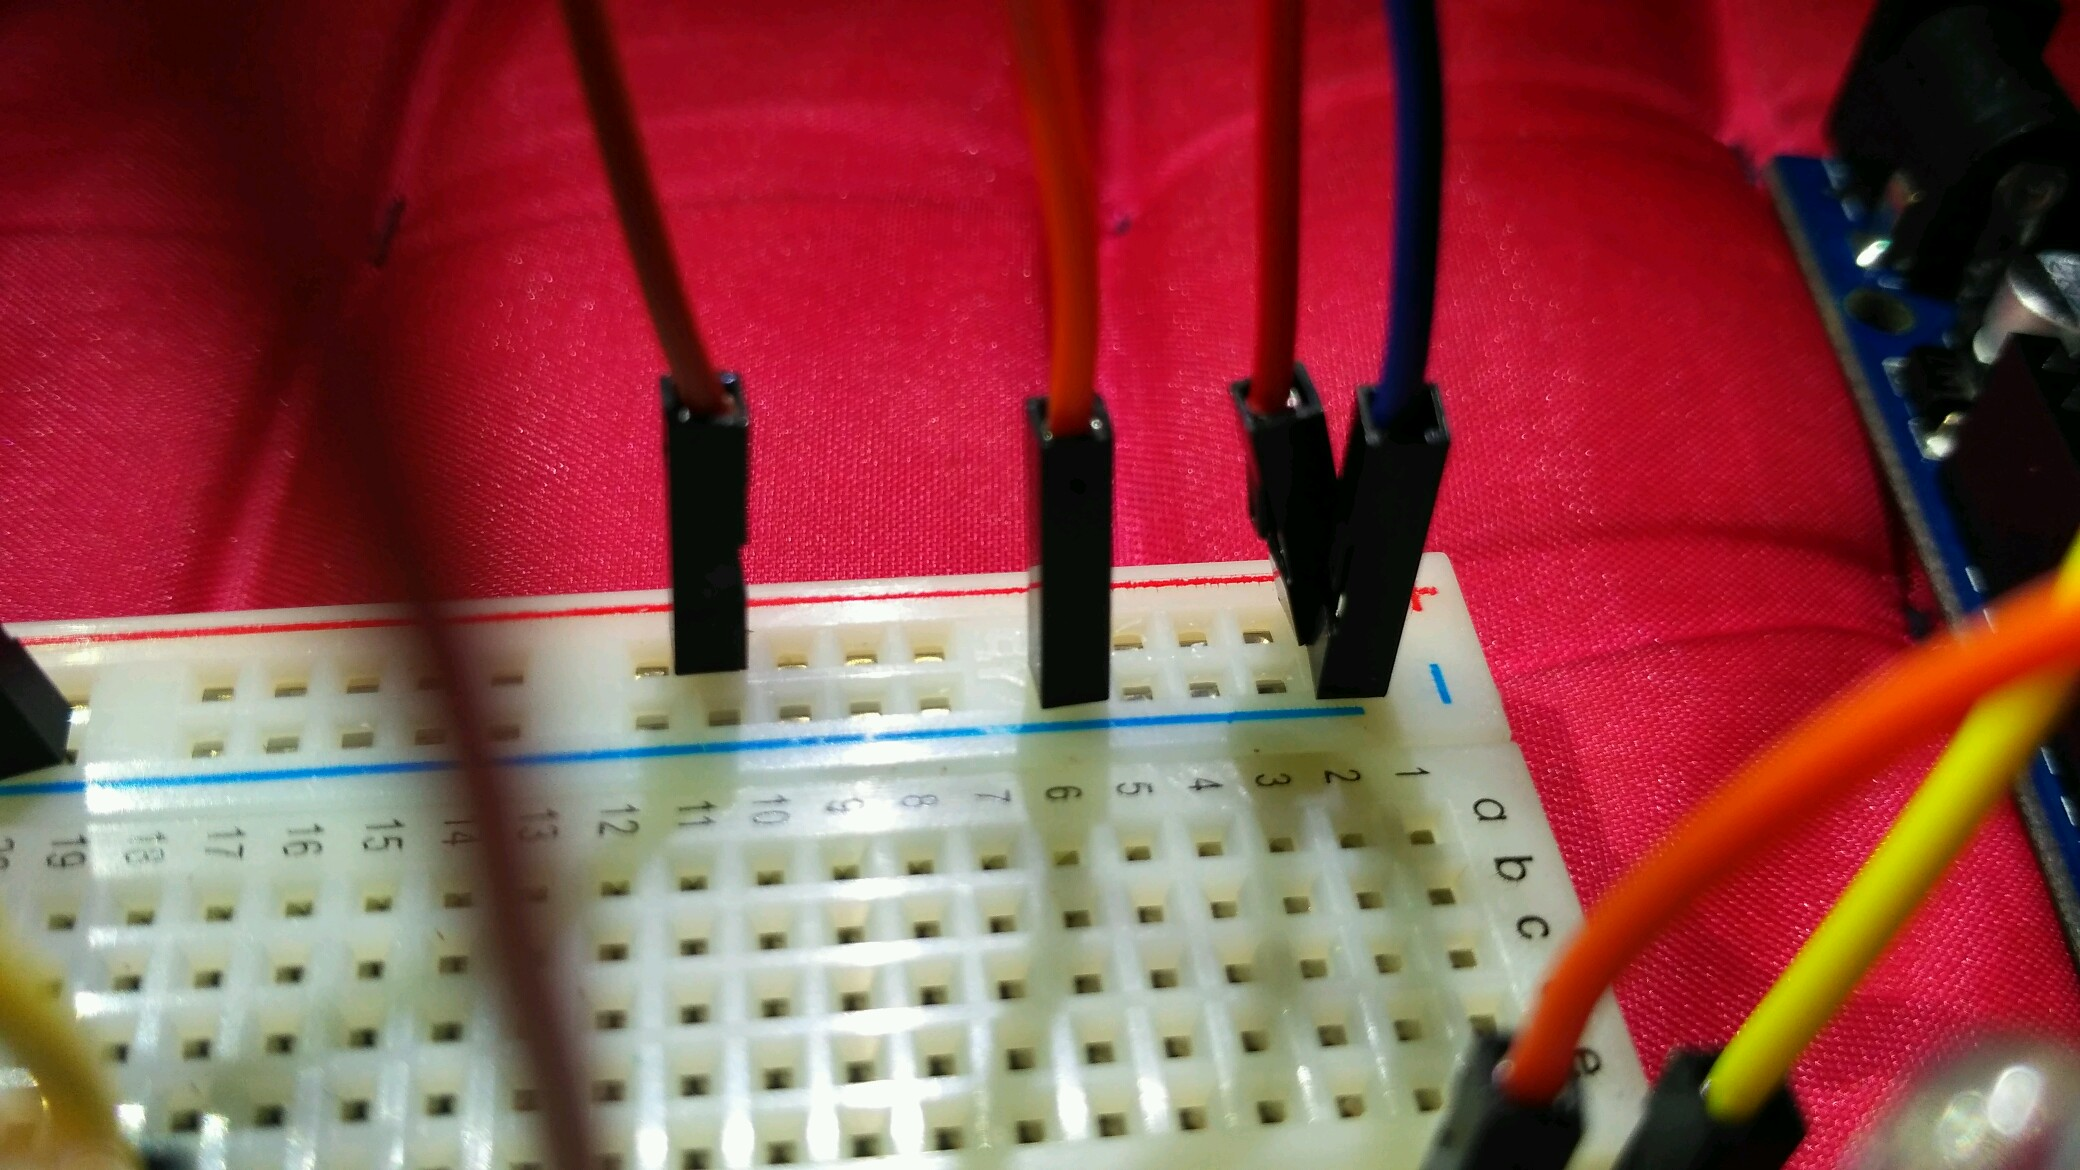
\includegraphics[width=0.9\textwidth]{figures/16.jpg}}
	\break
	\item tampilan setelah semua kabel terpasang.
	\break
	\centerline{\includegraphics[width=0.9\textwidth]{figures/17.jpg}}
	\break
	\item kemudian pasang kabel usb pada arduino dan laptop/komputer
	\break
	\item tahap terakhir buat program yang sesuai dengan sensornya lalu upload program tersebut pada arduino.


	
\end{enumerate}

\end{document}